\chapter{Related Work}
\label{chap2:related_work}

The goal of the present chapter is to provide a review of the most relevant ideas and techniques in the areas of interest. To that end, the following sections are organised as follows: section \ref{sec:chap2_biometric_recognition} starts by acknowledging and describing our domain (i.e., biometric recognition); section \ref{sec:chap2_deep_learning} describes the concepts behind \ac{DL}, as well as, its most popular architectures (like \ac{CNN}s and \ac{GAN}s); section \ref{sec:chap2_machine_learning_explainability} follows up by compiling a list of techniques that are commonly cited in the field of Explainability; section \ref{sec:chap2_conclusion} summarises the key aspects of this chapter.

\section{Biometric Recognition}
\label{sec:chap2_biometric_recognition}

Typically, a recognition problem involves a set of unique and non-transferable features that can unmistakably identify a subject. Biometrics, as they are usually designated, serve such purposes, as long as they are universal, distinguishable, resilient to changes and relatively easy to collect \cite{introduction_to_biometric_recognition}. 

Upon proving their compliance with these requirements, biometrics can be used to uniquely identify instances of data. 
Naturally, not every biometric suits every use case, and it is an engineering problem to determine which traits will likely convey the highest success rates. Amongst the varied set of possible biometric signals, the following remain the most popular:

\begin{itemize}
    \item \textbf{Face}: face recognition has the natural advantage of being largely non-intrusive (i.e., it can work in both controlled and uncontrolled environments), by usually focusing on the location and shape of facial attributes. Unfortunately, certain lighting conditions or unfavourable capture angles make it  more challenging to identify people by exclusively relying on facial data.
    \item \textbf{Iris}: iris recognition relies on the complex, yet unique patterns of an individual's iris. These can be captured with both visible and near infrared wavelength cameras, to highlight the colour and structure of the iris, respectively. Additionally, it is quite difficult to wittingly alter an iris' textures or use an artificial iris altogether, making this trait a solid candidate for many real world applications.
    \item \textbf{Fingerprint}: fingerprint recognition has also been preferred for a wide range of applications, by asking the user to place one or multiple fingers on top of a dedicated scanner. The ridges and valleys on the fingertip are so unique that each finger from the same person has different information. Although more common and less expensive, fingerprint based solutions are still sensitive to external conditions like debris, cuts or bruises on one's fingertip (not to mention gloves).
    \item \textbf{Gait}: gait recognition differs from the biometrics above because it requires both spatial and temporal information, so as to analyse the way someone walks. In practice, the movement patterns of a person's joints, when walking, can be seen as unique and invariant enough to constitute a biometric (if not for anatomic changes that our bodies endure over time). Unfortunately, processing gait information is computationally expensive, requires more physical space and does not offer the same accuracy levels that other traits do.
    \item \textbf{Voice}: voice recognition is, just like gait, an action over time (i.e., a subject must record a voice clip for subsequent processing). Our ability to speak is conditioned by anatomic properties (e.g., vocal tract, mouth) and therefore contains useful information. Despite this, the widespread adoption of such systems remains largely held back by voice altering factors (e.g., catching a common cold or having a hoarse voice).
\end{itemize}

Furthermore, these unique traits can be divided into two major categories: $\mathbf{1}$) \textit{physiological} biometrics (e.g., the iris, fingerprint and retina) that are naturally possessed by a given subject and $\mathbf{2}$) \textit{behavioural} biometrics (e.g., the gait and handwritten signature) that yield from the interaction between a subject and the surrounding environment  \cite{biometric_recognition_dl_survey}.

\subsection{Periocular Recognition}
\label{subsec:chap2_periocular_recognition}

Concentrating growing interests in the biometrics domain, periocular recognition uses the information in the vicinity of the eye, in which the iris, sclera, eyebrow, eyelid and skin stand out. \\

The seminal breakthroughs in the aforementioned area can be traced back to a set of methods termed "feature descriptors". Methods such as \ac{HOG}, \ac{LBP} and \ac{SIFT} were able to produce simplified data representations by relying on edges, textures and keypoints, respectively. In \cite{feasibility_study}, the results from each feature descriptor were fused to faithfully discriminate between the ''genuine''/''impostor'' pairs. This work served as the basis for subsequent fusion-based approaches, as in \cite{information_fusion_approach}.  In \cite{rbm_feature_learning} a Restricted Boltzmann Machine was used to learn a probabilistic distribution over the input data, further discriminated with metric learning and \ac{SVM}s.\\

With the effective application of \ac{DL} solutions, researchers turned to popular architectures (in particular \ac{CNN}s), to pursue ever increasing recognition accuracy. Accordingly, in \cite{accurate_periocular_recognition} the main concept involves the use of multiple \ac{CNN}s that are specialised in classifying a particular kind of semantic information (e.g., gender or age). Then, a score fusion process yields the final response. In \cite{deep_prwis},  authors enforce a \ac{CNN} to ignore the ocular region (due to its likelihood to contain specular reflections) and rely on the eye's surrounding area (eyebrow, eyelid and skin). \cite{person_identification} created independent representations of the iris and periocular regions, that feed classification modules, whose scores are finally fused to reach the decision. Using a multi-glance mechanism, where part of the intermediate components are configured to incorporate emphasis on the most important semantical regions (i.e., eyebrow and eye), Zhao and Kumar~\cite{zhao_kumar_novel} developed a recognition model that particularly focuses on these regions, enabling the deep \ac{CNN} to learn additional discriminative features that improve the recognition ability of the whole model. 

Recently, \cite{towards_interpretable_face_recognition} attempted to bridge the gap between biometric recognition and explainability, by learning feature specific filters that respond in their preferred spatial locations. 

Finally, \cite{interpretability_by_parts} propose an integrated solution that leverages the discovery of parts as a form of attention. More specifically, a dictionary of object parts is learned, upon which a feature map can be grouped into part segments. Then, an attention mechanism determines the parts that should be regarded as essential to the classification process. This solution (hereby referred to as HL) is similar to our methods with respect to the integration of explainability into a recognition framework, making it a prime candidate for a direct comparison (as seen in section \ref{subsec:chap4_explainability_evaluation}).

\section{Deep Learning}
\label{sec:chap2_deep_learning}

As a subordinate area to \ac{ML}, \ac{DL} focuses primarily on algorithms that mimic the human brain and how the seemingly simple neurons receive, process, store and release information in a coordinated manner.  Fortunately, the field has progressed immensely throughout the years, updating and rethinking its archetype (i.e., \ac{ANN}s) to perform a wide range of tasks. However, despite the groundbreaking success of these approaches, the field went through some really unremarkable periods before becoming so coveted as it is nowadays.\\

The first efforts in the field of \ac{DL} can be traced back to $1943$, with the work of neuroscientist Walter Pitts and mathematician Warren McCulloch. They proposed the simplest of elements, one that did so little but, when combined with more of its kind, could achieve a whole much greater than the sum of its parts. The artificial neuron was capable of taking inputs, assigning weights to them and, through some light processing, reach an output.

More than a decade after the first steps, the next major innovation came in the form of the Perceptron \cite{perceptron}, so called by Frank Rosenblatt, its inventor. This algorithm could be used to solve linearly separable binary problems, in a supervised manner (i.e., the training samples possess ground-truth labels, against which the model's predictions are to be compared). Some relevant concepts were established, like the use of activation functions to give more expressive power.
Moreover, this work started with a single layer Perceptron and naturally extended to an \ac{MLP} (i.e., multiple layers of these units). A formulation similar to this one is still used in modern architectures, whether in a feed-forward style, where connections between nodes do not form cycles, or otherwise (i.e., \ac{RNN}s).

The next couple of decades marked the first really low point in the field's research interest, except for the continued work upon the ideas behind Perceptrons and the discovery of the backpropagation algorithm in $1974$ (the default procedure for weight optimisation, based on the derivative of a loss function with respect to a given weight).

After this period, research saw a rejuvenated wave of interest, with breakthroughs like the formalisation of the \ac{CNN}'s precursor, the Neocognitron \cite{neocognitron}. Kunihiko Fukushima described such framework, in $1980$, as having two basic types of layers: convolutional and downsampling/pooling layers. Convolutional layers would serve the purpose of applying a sliding window (i.e., a kernel with learnable weights) over the input to extract features. Downsampling layers, usually in between convolutional layers, could reduce the spatial complexity of the input and, as a side benefit, give invariance to a feature's occurrence. 

In $1989$, Yann LeCun, one of the better known individuals in the \ac{DL} community, combined a \ac{CNN} with backpropagation to classify handwritten digits. Subsequent work led to the establishment of one of the most relevant \ac{ANN} designs, LeNet$5$ \cite{lenet5}.

Several years later, the next \ac{DL} revolution was made possible by the advent of \ac{GPU}s, reducing training times to much more realistic amounts. Based on that, Alex Krizhevsky, under the supervision of another \ac{DL} great, Geoffrey Hinton, proposed AlexNet \cite{alexnet} and achieved a record top-$5$ error in \ac{ILSVRC}-$2012$, proving that deep \ac{CNN}s were feasible and well suited to the image classification task. Moreover, it showed that \ac{ReLU} could be amongst the \textit{de facto} activation functions.

Whilst the \ac{DL} revolution was put in motion, areas like Image Segmentation saw an uprising of novel methods, diverging from the classical clustering or colour/edge based segmentation methods. Many of those methods became obsolete, as the state-of-the-art moved on to fully connected and region-based approaches \cite{review_of_semantic_segmentation}.

Another recent line of work has to do with generative algorithms, brought forward in the original \ac{GAN} paper \cite{goodfellow}, co-authored by Ian Goodfellow and Yoshua Bengio, the third pioneer of \ac{DL}. \\

Outside of the theoretical strides, practitioners and newcomers have enjoyed the success of specialised frameworks that grant more mainstream appeal to \ac{DL} as a whole. Tensorflow \cite{tensorflow} and PyTorch \cite{pytorch} are two of those tools, with similarities and disparities that make them more suited to different target audiences. Nonetheless, both include \ac{API}s that make the coding more user friendly.\\

For the purposes of this work, algorithms like \ac{CNN}s and \ac{GAN}s, amongst others, are of particular interest. Therefore, the following subsections describe those architectures both in general and, through the actual models that were chosen, in particular.

\subsection{Convolutional Neural Networks}
\label{subsec:chap2_cnn}

As mentioned above, \ac{CNN}s have the ability to take a fixed-size image as input, apply complex operations and determine the corresponding class (i.e., the group it belongs to). A typical \ac{CNN} architecture includes a feature extraction stage and a classification stage. The first analyses the image to keep the core aspects, while the second translates that information into the predicted class. The image below is a visual representation of what was described in this paragraph:

\begin{figure}[h]
\centering
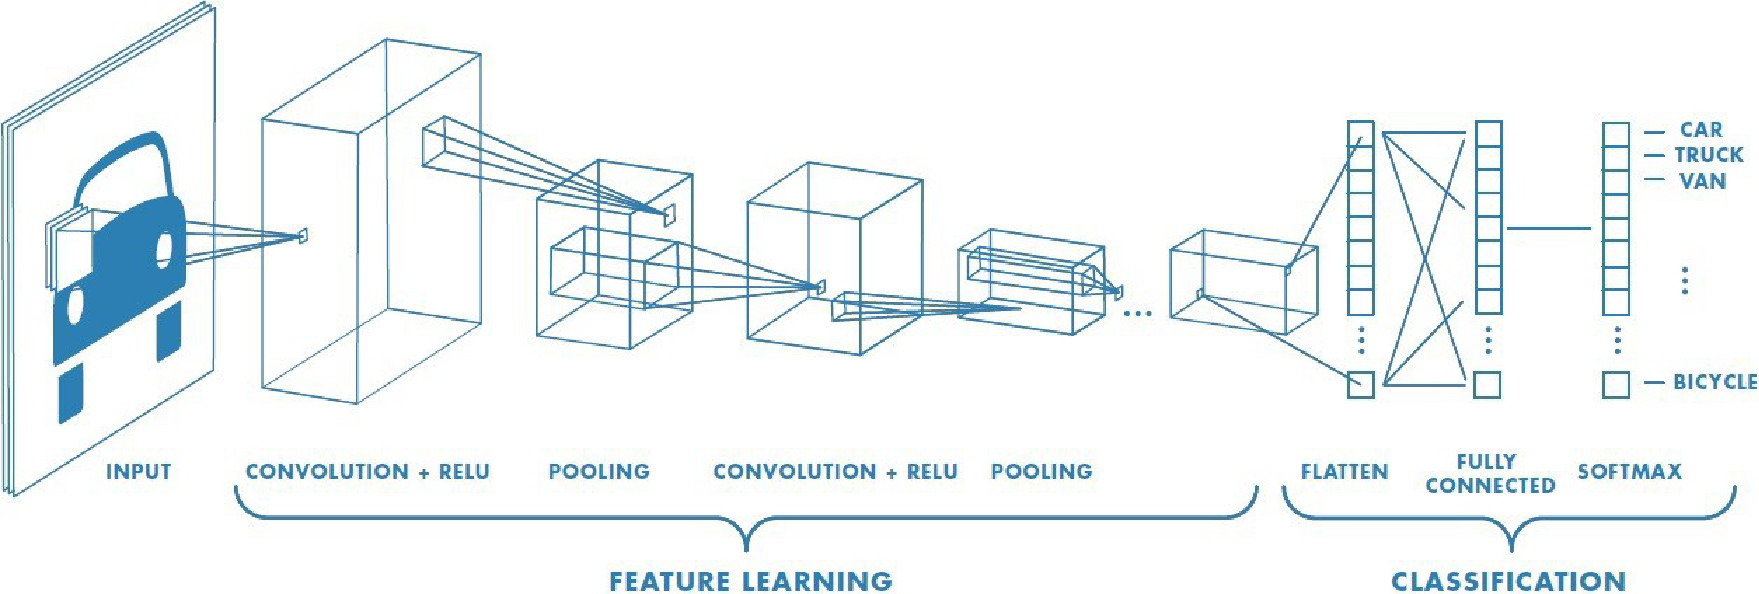
\includegraphics[width=380pt]{figures/figure_2.pdf}
\caption{Typical \ac{CNN} architecture \cite{cnn_architecture}. The feature extraction stage extracts as many characteristics as possible from the input image, while the classification stage gives them meaning (i.e., a class).}
\label{fig:cnn}
\end{figure}

During the feature extraction stage, the image goes through a series of convolutional and pooling layers. A convolutional layer contains a certain number of filters/kernels of small size (e.g., $3$x$3$ or $5$x$5$ pixels). These filters are responsible for learning both low and high level features from the source image. The first layers usually capture lines, curves and general shapes, while the deeper ones are able to capture more and more abstract concepts. As Fig. \ref{fig:cnn} shows, a filter is a small window that slides over the input, multiplying its values (learned weights) by the ones from the input.
    
In between convolutional layers, pooling layers are responsible for reducing the dimensionality of the previous layer's output (in Fig. \ref{fig:cnn}, every time a pooling operation is performed, the input's height and width are reduced, with the depth being determined by the number of filters). This step also ensures that a feature's occurrence is spatially invariant. Just like convolutional layers, pooling layers use a kernel of size $N$x$N$, but unlike convolutional layers, they doesn't possess learnable weights. Two commonly used forms of pooling are max-pooling and average-pooling: the former only keeps the biggest value inside the chosen kernel, while the latter keeps the mean of all the values inside the kernel.\\
    
After extracting features from the input image, the final feature maps are flattened (i.e., stretched to a vector like shape) and fed to a regular \ac{MLP}. An \ac{MLP}, as described earlier, is a sequence of \ac{FC} layers of neurons, meaning that a neuron receives the output of every neuron, in the previous layer, and its output is sent to every neuron in the next layer.
    
Finally, the output layer (last layer of neurons) has, typically, a neuron for each class and the values given by those neurons are the probability of the input image belonging to the classes associated with those neurons (i.e., in Fig. \ref{fig:cnn}, the first neuron outputs the probability of the image belonging to the "car" class).\\

Within convolutions and neurons, there are special functions (called "activation functions" in the literature) that usually perform non-linear operations. 

In convolutions, an example could be the \ac{ReLU} function, which simply maps negative inputs to zero and behaves like the identity function for positive ones. 
    
Neurons, on the other hand, receive several inputs and perform a weighted sum with them (once again, these weights are the parameters learned by the network). Next, the result is given to an activation function (like \ac{ReLU}, sigmoid or softmax, as shown in Fig. \ref{fig:cnn}), which determines the neuron's activation value.

These kinds of functions are crucial, without them a neuron could only process simple data, and not complex (non-linear) data, like images.\\

Understandably, these methods have been at the core of research efforts over the past years, not only for their ability to learn meaningful information but also due to the democratisation of \ac{GPU}s. Naturally, many deep designs were proposed, including the Inception \cite{inception}, VGG \cite{vgg}, ResNet \cite{resnet} and DenseNet \cite{densenet} architectures (which subsection \ref{subsubsec:chap2_densenet} covers in more detail).

\subsubsection{DenseNet}
\label{subsubsec:chap2_densenet}

Throughout the years, \ac{CNN}s got deeper and deeper, in a move that the research community saw as somewhat natural. In spite of this, the gradient based training seemed to halt this trend. That situation was addressed by the ResNet design, which introduced residual connections to create information pathways between more layers, thus controlling the vanishing gradient problem. Additionally, the work with such deep networks showed how some layers could be dropped during training while not seriously affecting the overall performance. Hence, there was evidence that deep residual networks possess a great deal of redundancy \cite{densenet, deep_residual}. Based on this knowledge, the authors of DenseNet proposed an architecture similar to the following: \\

\begin{figure}[h]
\centering
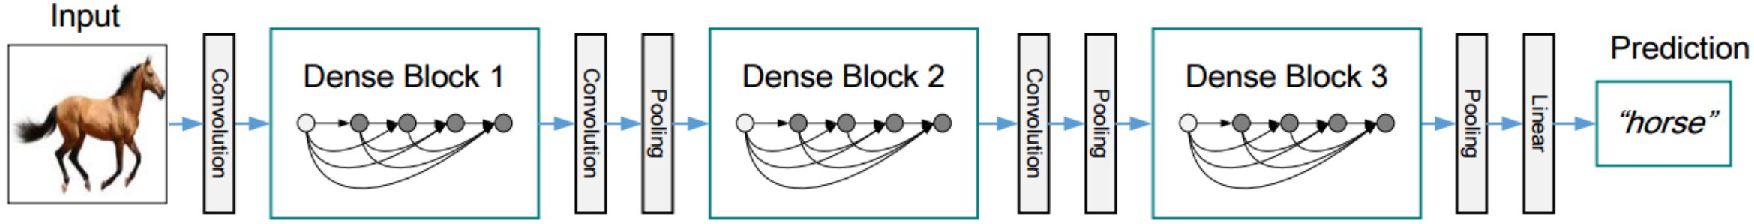
\includegraphics[width=390pt]{figures/figure_3.pdf}
\caption{Deep DenseNet with three dense blocks \cite{densenet}. Each one of those blocks contains a series of convolutions, pooling and/or \ac{BN} layers.}
\label{fig:densenet}
\end{figure}

Fig. \ref{fig:densenet} contains an example of a deep DenseNet with three blocks, each containing 5 layers. The circles represent the feature maps and the arrows send them through composite functions of operations (including \ac{BN}, convolutions and pooling), which output more feature maps. Due to the many connections, each composition of operations receives a concatenation of every feature map from the previous layers. In between dense blocks, we have the so called "transition layers", which change the feature maps' sizes via convolution and pooling operations. 

With this approach to network design, the authors gave the model a set of densely packed blocks to perform the feature extraction process. Naturally, many versions of the same design were created, like DenseNet-$121$, DenseNet-$161$ or DenseNet-$201$ (where the number is analogous to the number of layers that were included).

\subsection{Region-based Instance Segmentation}
\label{subsec:chap2_region_based_instance_segmentation}

The basic idea behind image segmentation comes from the definition of the word "segmentation": division into separate parts/sections. With effect, when an algorithm attempts to segment an image, it tries to determine the object that a given pixel belongs to. Notice the wording here, because, unlike object detection, a segmentation algorithm does not need to know what the objects and visual elements represent (i.e., the classes). But before we discuss instance segmentation, we should create a notion for object detection first. 

\subsubsection{\ac{R-CNN}}
\label{subsubsec:chap2_rcnn}

The region-based family of object detection algorithms relies on the proposal of \ac{RoI} in any given image. A naive approach to this task would be to consider all possible bounding boxes, with varying dimensions, aspect ratios and positions. Unfortunately, this algorithm would rapidly become prohibitive in terms of the computational budget. So, to keep the same idea but make it more efficient, the \ac{R-CNN} paper \cite{r_cnn} used selective search \cite{selective_search} to consider just a few thousand region proposals. The following steps and Fig. \ref{fig:selective_search} provide more details on how the proposals are derived:

\begin{enumerate}
    \item Start with an initial set of seemingly random segmentation regions.
    \item Group neighbouring regions together, based on a number of similarity metrics (e.g., colour, texture or size).
    \item Repeat the previous step until the stopping criterion is reached (e.g., maximum number of iterations).
\end{enumerate}

\begin{figure}[h]
\centering
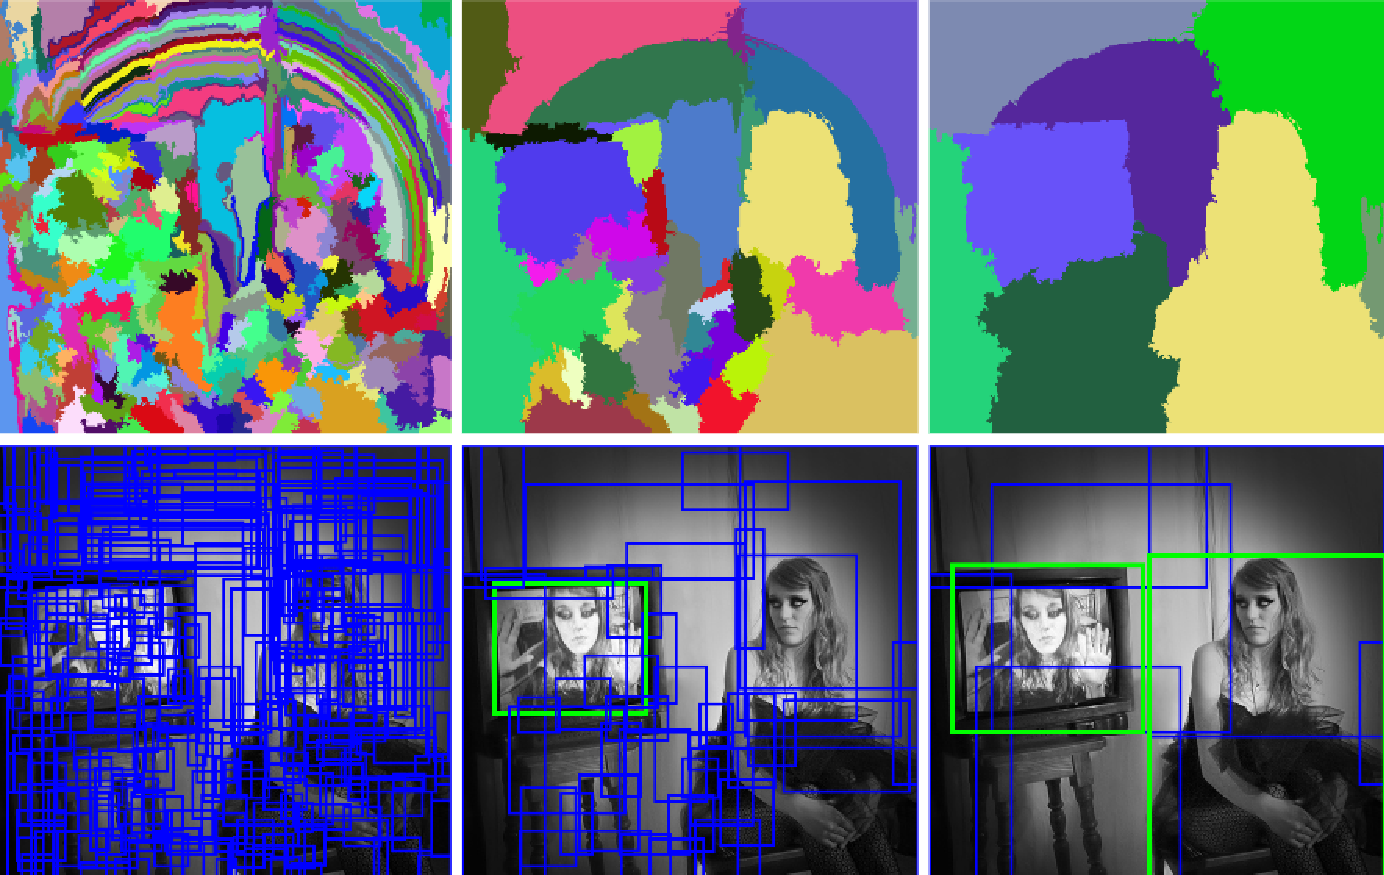
\includegraphics[width=0.8\textwidth]{figures/figure_4.pdf}
\caption{Visualisation of how the selective search algorithm progresses \cite{selective_search}. The top row contains the segmented regions, while the bottom row contains the corresponding bounding boxes. The algorithm works by joining similar regions together until a stopping condition is reached.}
\label{fig:selective_search}
\end{figure}

Next, the region proposals are resized to a square aspect ratio and fed to a \ac{CNN} that acts as a feature extractor. Finally, for each region proposal, a trained \ac{SVM} receives the corresponding feature maps (which are flattened to become a $4096$-dimensional vector) and detects the presence of any object of the class it was trained on:

\begin{figure}[h]
\centering
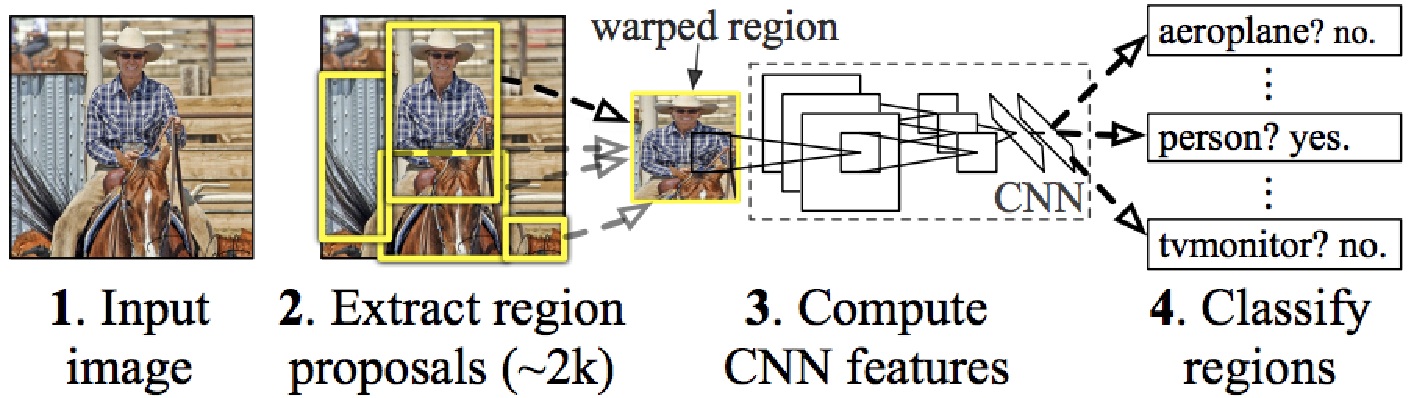
\includegraphics[width=325pt]{figures/figure_5.pdf}
\caption{\ac{R-CNN} pipeline \cite{r_cnn}. The framework uses selective search to create region proposals, which are later fed to a \ac{CNN} that extracts features. Then, a trained \ac{SVM} classifies the feature maps as describing a known object or not.}
\label{fig:r_cnn}
\end{figure}

\subsubsection{Fast \ac{R-CNN}}
\label{subsubsec:chap2_fast_rcnn}

After the publication of the \ac{R-CNN} paper, one of the authors improved the architecture with Fast \ac{R-CNN} \cite{fast_r_cnn}, a much faster and accurate approach. This new version still relies on selective search to generate region proposals but includes some key improvements.\\

Once the region proposals (i.e., \ac{RoI}) are generated, the image is fed to a \ac{CNN} responsible for extracting a single set of feature maps. Then, each \ac{RoI} is projected in the common feature maps,  effectively slicing it into smaller feature maps. Next, a new layer called \ac{RoIPool} computes a fixed-length vector for each \ac{RoI}: it applies max-pooling to each slice of feature maps, ensuring a pre-defined $H$x$W$ size, thus creating a small feature map for every \ac{RoI} that still relies on shared computations. Here we start to see the gains in speed and space by only extracting features once. The pipeline continues by mapping the smaller, \ac{RoI} specific, feature maps to a feature vector, using \ac{FC} layers. Finally, the architecture bifurcates into two branches with additional \ac{FC} layers: one serves the classification purposes and has a "$K + 1$"-way softmax, with probabilities for each of the $K$ classes and the "background" class; and another performs regression by outputting four values for each class, representing the bounding box corners:\\

\begin{figure}[h]
\centering
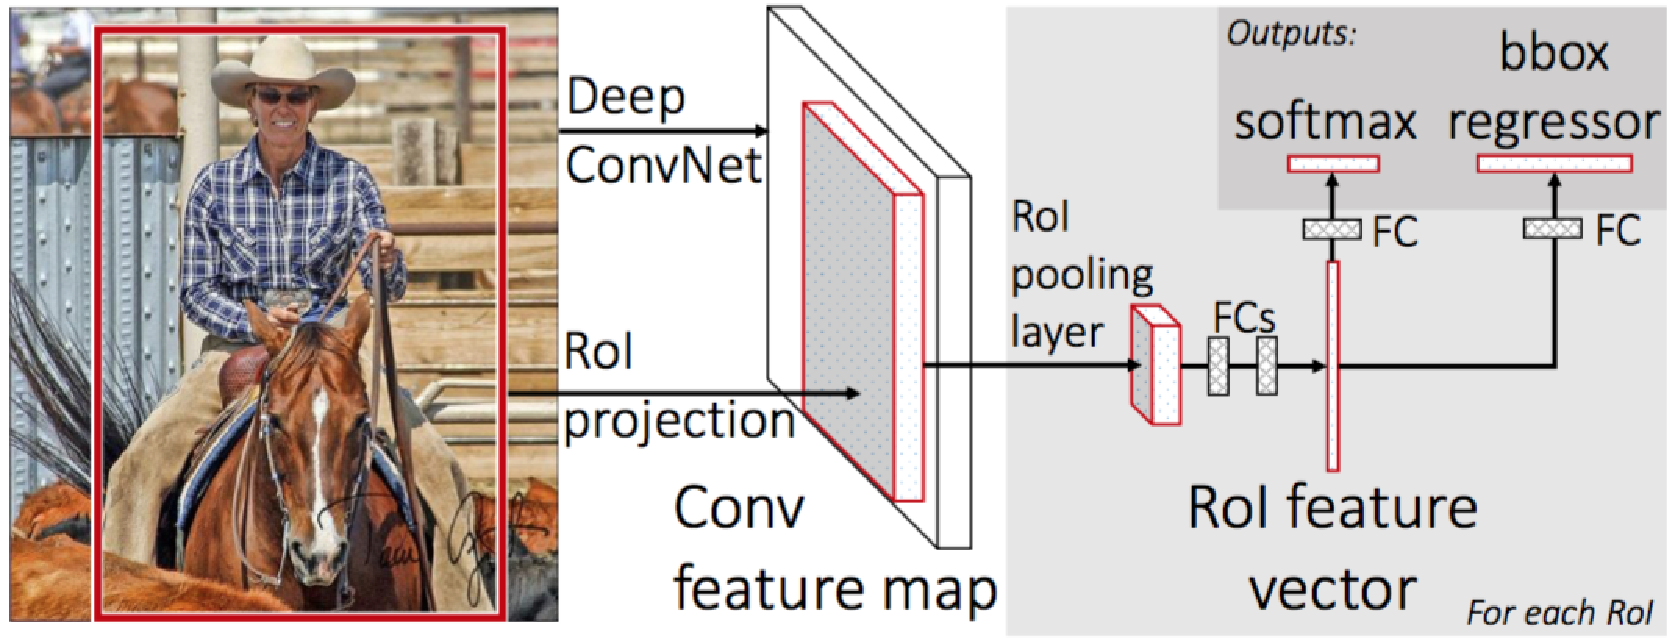
\includegraphics[width=260pt]{figures/figure_6.pdf}
\caption{Fast \ac{R-CNN} pipeline \cite{fast_r_cnn}. The revision of \ac{R-CNN} uses a common feature map, shared by all region proposals, instead of extracting features for each and every proposal.}
\label{fig:fast_r_cnn}
\end{figure}

\subsubsection{Faster \ac{R-CNN}}
\label{subsubsec:chap2_faster_rcnn}

Making further improvements, the Faster \ac{R-CNN} \cite{faster_r_cnn} architecture extends the Fast \ac{R-CNN} predecessor by replacing the mechanism that proposes the object regions. Faster inference times and accuracy are, once again, made possible by some rethinking of the core aspects. Two modules serve as the basis for this unified framework: \ac{RPN} and Fast \ac{R-CNN} detector. The following figure contains a good visual approximation of the Faster \ac{R-CNN} architecture:

\begin{figure}[h]
\centering
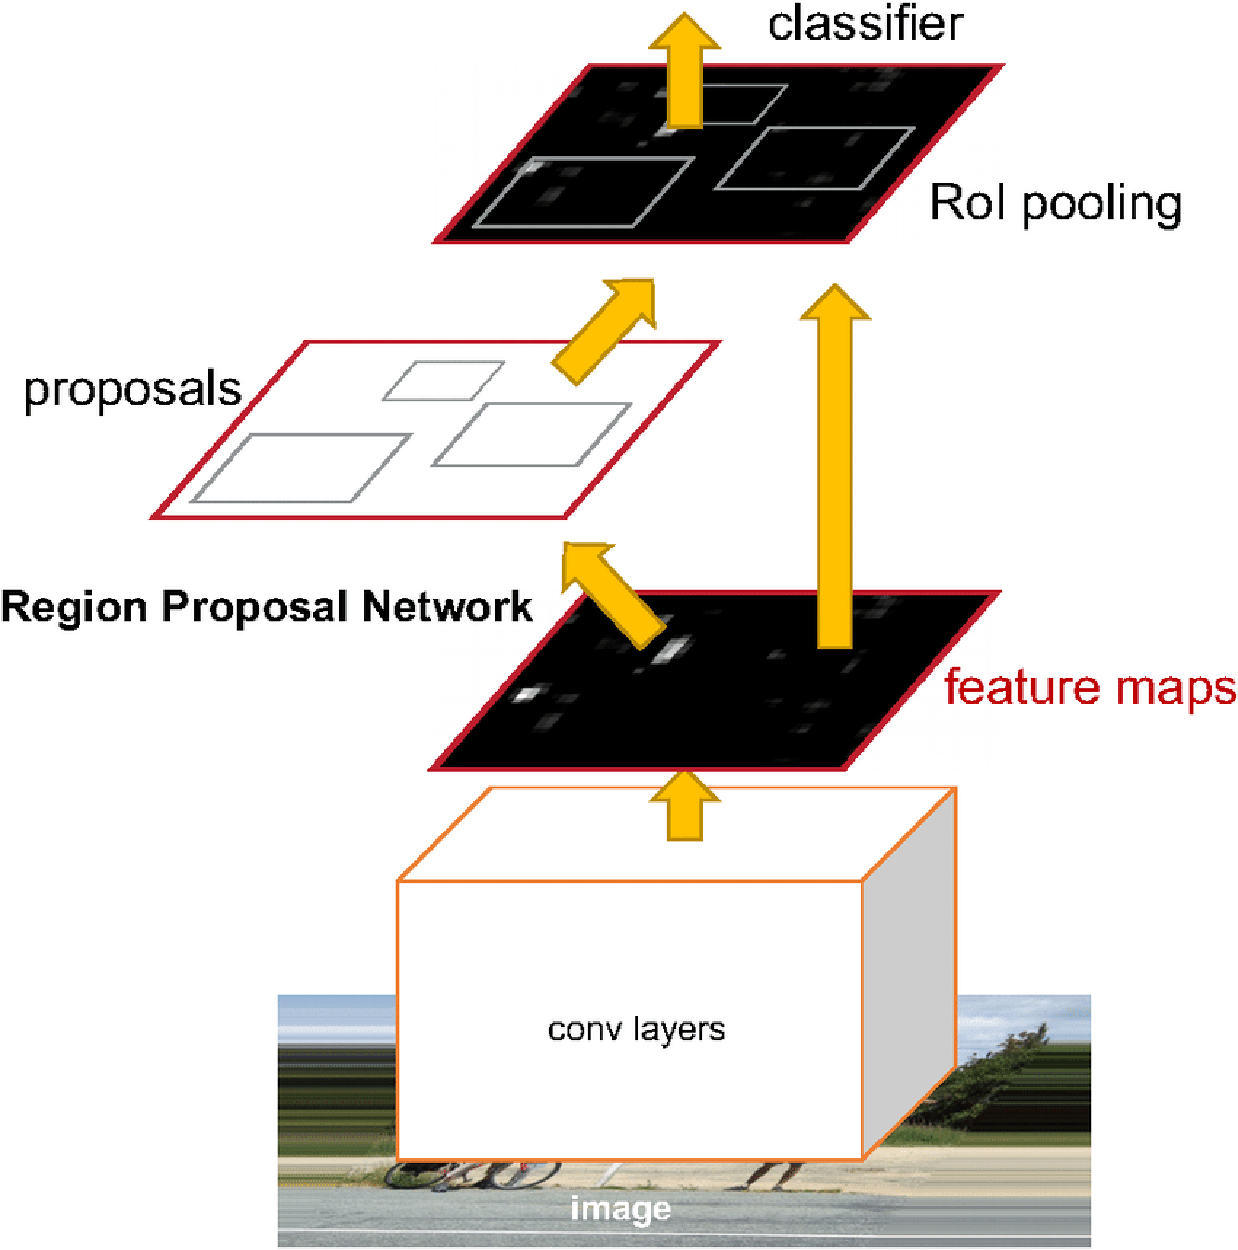
\includegraphics[width=170pt]{figures/figure_7.pdf}
\caption{Faster \ac{R-CNN} pipeline \cite{faster_r_cnn}. The two main modules are the \ac{RPN}, to predict where an object might be, and the \ac{R-CNN} detector, to classify the proposed regions.}
\label{fig:faster_r_cnn}
\end{figure}

The advantages brought forward by the \ac{RPN} include its speed and the  ability to be tuned to a specific task (i.e., because it is a trainable component, it can become better suited to the types of images and biases in the training set, unlike generic algorithms like selective search). The \ac{RPN} works by using $k$ anchor boxes (which are, essentially, matrices of varying aspect ratios) that slide over the image's feature maps, followed by an intermediate layer that produces a fixed-length vector (e.g., $256$-dimensional) for each anchor. This vector is then given to two separate \ac{FC} branches. On one hand, the first branch outputs $2k$ scores (two for each of the $k$ anchors) which are the probabilities of an object's presence in each proposal. On the other hand, the second branch outputs four bounding box coordinates for each of those $k$ anchors: 

\begin{figure}[h]
\centering
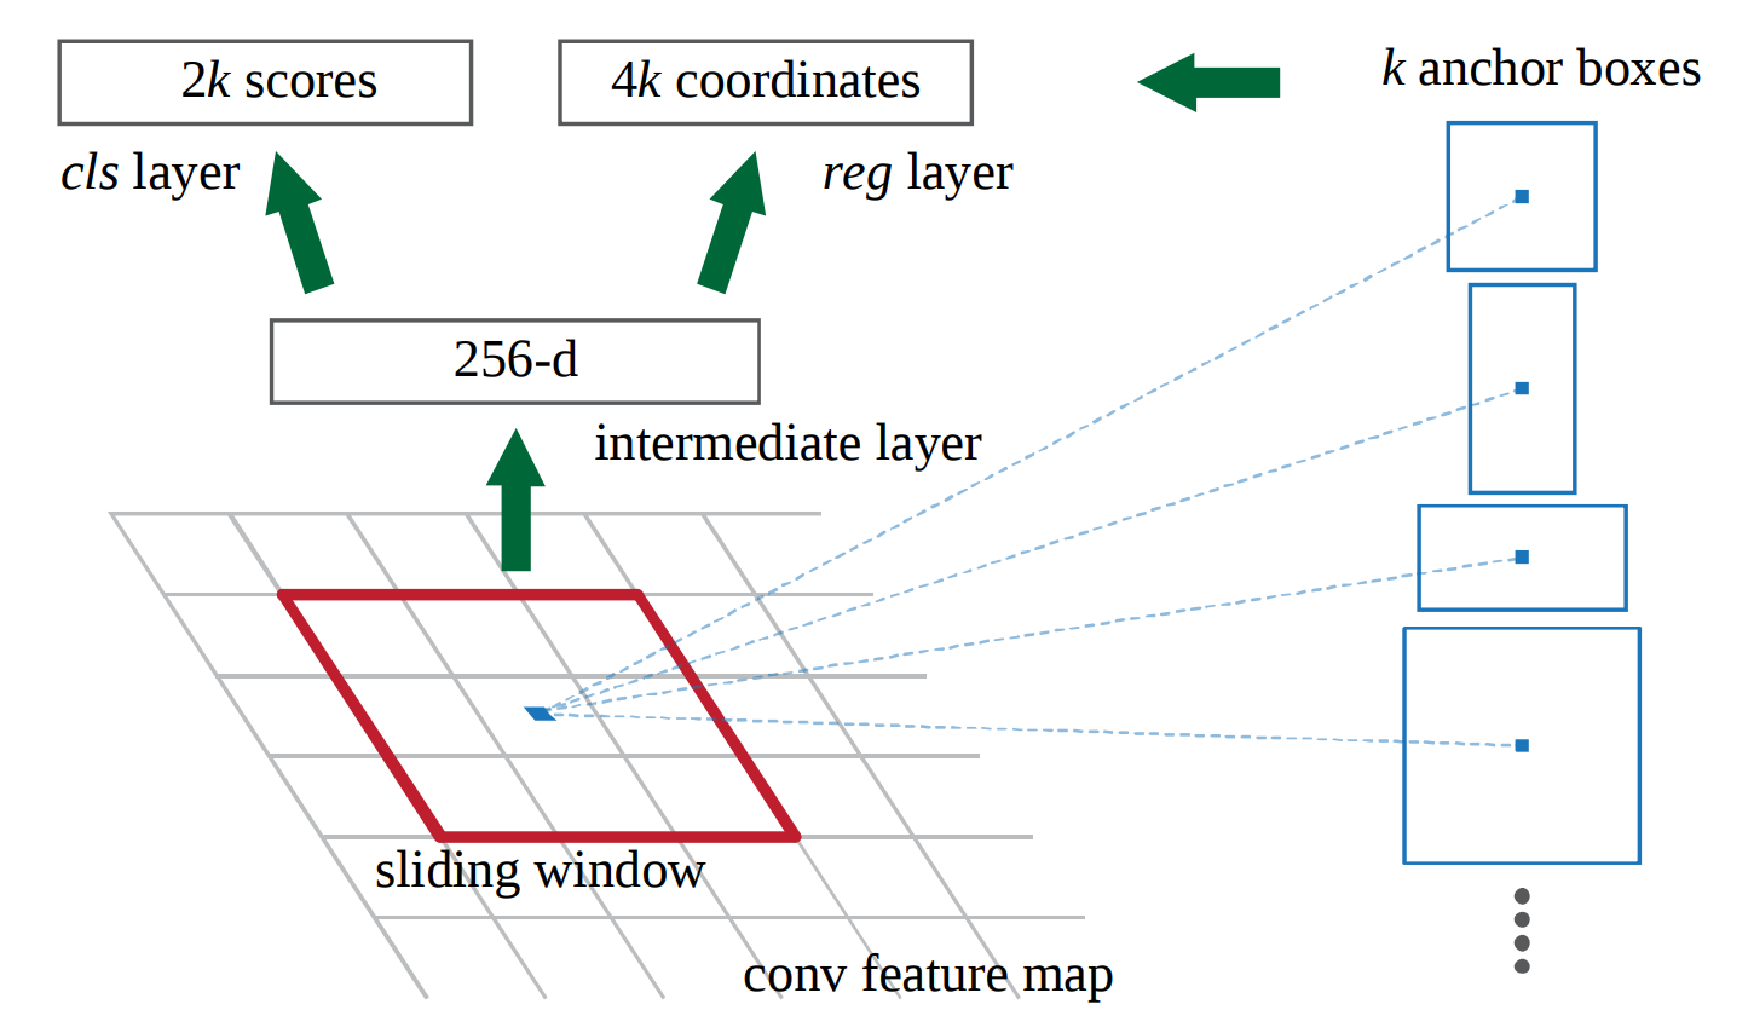
\includegraphics[width=215pt]{figures/figure_8.pdf}
\caption{Visualisation of the proposed \ac{RPN} \cite{faster_r_cnn}. By using multiple anchors with different aspect ratios and sliding them over the received feature maps, the network is able to extract several fixed-length vectors, which are later used for classification and regression.}
\label{fig:faster_r_cnn_rpn}
\end{figure}

With the region proposals and the image feature maps (the same used by the \ac{RPN} module), the Fast \ac{R-CNN} detector can find the slice of feature maps that correspond to each region proposal and pass it through the \ac{RoIPool} layer. Then, just like before, a \ac{RoI} feature vector is computed using a couple of \ac{FC} layers and given to two sibling branches, which output a class and bounding box. \\

With the architecture assembled, all that is needed is a way to train it. To do so, the authors propose a $4$-step training procedure: 

\begin{enumerate}
    \item The \ac{RPN} is initialised with ImageNet weights and fine-tuned to perform the region proposal task.
    \item With the generated proposals from step $1$, the Fast \ac{R-CNN} detector is also fine-tuned with ImageNet weights.
    \item The convolutional layers that extract features from the original image are initialised with the Fast \ac{R-CNN} weights (remember that these layers are shared across \ac{RPN} and Fast \ac{R-CNN}). The remaining unique layers of the \ac{RPN} are fine-tuned.
    \item Finally, keeping the shared convolutional layers fixed (from step $3$), the unique layers of Fast \ac{R-CNN} are fine-tuned, resulting in a trained and unified framework.
\end{enumerate}

Faster \ac{R-CNN} achieved state-of-the-art performance in popular datasets like Pascal \ac{VOC} and \ac{COCO}, remaining to this day as a very influential design.

\subsubsection{Mask \ac{R-CNN}}
\label{subsubsec:chap2_mask_rcnn}

Specifically designed to produce segmentation masks, the Mask \ac{R-CNN} framework \cite{mask_rcnn} is an extension of the previously discussed Faster \ac{R-CNN}. It adds a third branch to the already existing classification and bounding box regression ones. The mask branch is a small \ac{FCN} applied to each \ac{RoI}, resulting in the prediction of a binary mask:

\begin{figure}[h]
\centering
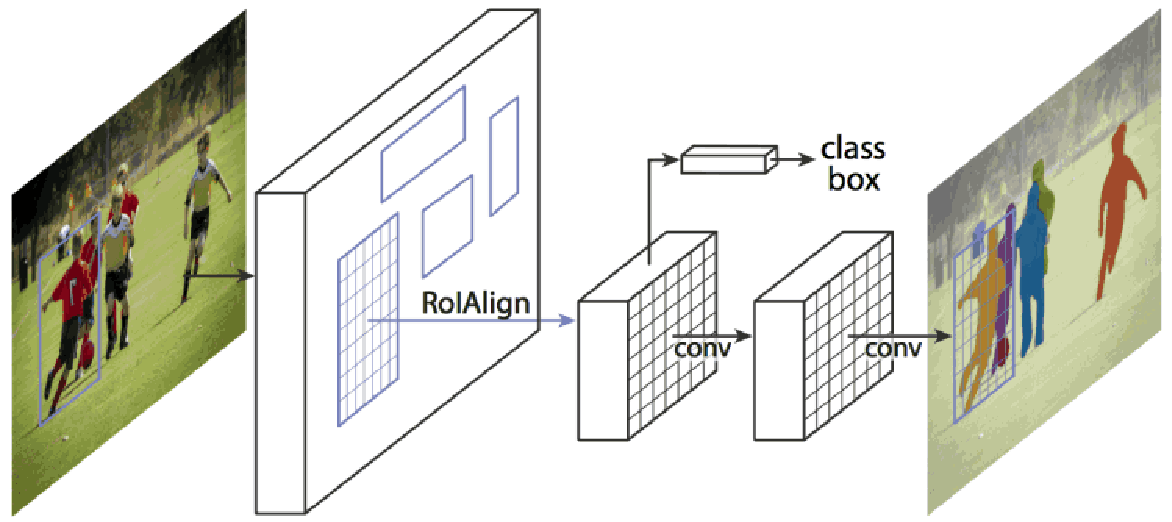
\includegraphics[width=300pt]{figures/figure_9.pdf}
\caption{Mask \ac{R-CNN} architecture \cite{mask_rcnn}. Built on top of Faster \ac{R-CNN}, this architecture favours segmentation and includes alignment techniques to ensure optimal mask quality.}
\label{fig:mask_r_cnn}
\end{figure}

By building on top of the Faster \ac{R-CNN} architecture, Mask \ac{R-CNN} adds very little extra overhead and keeps the speed that the former enjoyed. The \ac{RoIAlign} operation (depicted in Fig. \ref{fig:mask_r_cnn}), which fixes the \ac{RoI} misalignment present in the previous \ac{R-CNN} based methods, also helped the object detection performance (i.e., if the mask prediction branch is disabled, the resulting architecture behaves better than the baseline Faster \ac{R-CNN}). The reason for the misalignment in the original frameworks has to do with the approximations that are made with \ac{RoIPool}, resulting in the loss of some spatial information. \ac{RoIAlign}, on the other hand, does not use the exact values in the feature maps, but rather, interpolations that take into account the surrounding values. By doing so, we are using some of the information that would have been discarded by a quantisation based approach like \ac{RoIPool}. Only after doing this, can the max-pooling operation be used to obtain a fixed-size feature map (the maximum value still has some information about its surroundings).\\

Mask \ac{R-CNN} achieved, at the time, state-of-the-art results on the \ac{COCO} dataset and was even used to perform pose estimation, despite not being intentionally trained to do so.

\subsection{Generative Adversarial Networks}
\label{subsec:chap2_gan}

As generative algorithms, \ac{GAN}s possess the ability to create new data, unlocking many interesting possibilities. Although seemingly complex, the motivation behind these frameworks is really intuitive: two networks with competing goals are put against each other to make for a better learning process (i.e., if one gets better, the other has to keep up).\\

Formally, a generator $G$ tries to generate new data from random noise. Then, synthetic and real samples are given to a discriminator $D$, whose task is to distinguish their sources:

\begin{figure}[h]
\centering
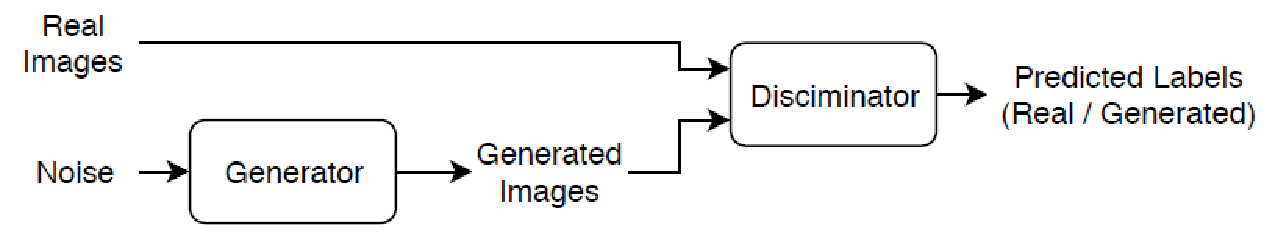
\includegraphics[width=360pt]{figures/figure_10.pdf}
\caption{Typical \ac{GAN} architecture \cite{gan_architecture}. The generator takes random noise as input and outputs fake, but realistic images. By the end of training, the fake images should be hard to distinguish from the real ones.}
\label{fig:gan}
\end{figure}

Analysing Fig. \ref{fig:gan}, one can understand the training process that much better: $G$ will learn to sample a random input vector and produce a synthetic image, so that it can fool $D$ into thinking it came from the real distribution. Conversely, $D$ will learn to distinguish fake samples from real ones. At first, $G$'s images will look nothing like the real ones, but the feedback loop will drive the two adversaries to a converged state: $G$ will be updated by how far it was from fooling $D$ and $D$'s update will be based on how it fared at discriminating between real and fake samples. After training, the discriminator is discarded and we are left with a generator that can produce realistic images.\\

Equations \ref{eq:1} and \ref{eq:2} present the formal loss functions that enable the training of both $D$ and $G$. It should be noted that, in the original description, $D$ will try to maximise the average of the log probability for real images, as well as, the log of the inverse probability for fake images. $G$, on the other hand, should seek to minimise the log of the inverse probability predicted by the discriminator for fake images:
\begin{equation}
    \mathcal{L}_D = \frac{1}{m}\sum_{i = 1}^{m}[\log(D(x_i)) + \log(1 - D(G(z_i)))]
    \label{eq:1}
\end{equation}
\begin{equation}
    \mathcal{L}_G = \frac{1}{m}\sum_{i = 1}^{m}\log(1 - D(G(z_i)))
    \label{eq:2}
\end{equation}
Since the original publication, the loss terms have been update, whether by making $G$ maximise the log of the discriminator probabilities for fake images or rethinking core aspects of the training procedure (as in Wassertein \ac{GAN}s \cite{wgan}, where the discriminator is replaced with a critic that scores how realistic the given samples look). Due to the high interest shown by the research community, many different designs were proposed, including Att\ac{GAN} \cite{attgan}, for image manipulation, and Style\ac{GAN}$2$ \cite{stylegan2}, for high quality image generation. Given its use in this work, the Style\ac{GAN} family is highlighted below.

\subsubsection{Style\ac{GAN}}
\label{subsubsec:chap2_stylegan_2}

The Style\ac{GAN} team started experimenting with a concept called "progressive growing". In the paper where they introduce this idea \cite{proggan}, the authors postulate that the discriminator $D$ and generator $G$ could start working with low resolution images (e.g., $4$x$4$ pixels) and then get progressively upgraded to deal with higher and higher resolutions. Both $D$ and $G$ would get new layers, at each resolution change, to deal with the higher dimensionality. To avoid the risk of sudden shocks or instability, the new layers are faded in smoothly and every layer remains trainable throughout the entire training process. This methodology allows both the $D$ and $G$ to first learn the large-scale aspects of the images and then, progressively, shift their attention to finer details, which usually come with higher resolutions. The resulting network, called Prog\ac{GAN}, was able to generate high quality images at higher than usual resolutions (e.g., $1024$x$1024$ pixels).\\

Following the work above, the same authors proposed an architecture called Style\ac{GAN}. The main differences between this architecture and the baseline Prog\ac{GAN} are the use of an additional mapping network to map latent codes to a new latent space, the use of style vectors and the introduction of \ac{AdaIN}. 

The mapping network opposes itself to the traditional \ac{GAN} formulation, where we map a point in the latent space to the image space. In this new configuration, we first map the latent points to an intermediate space, through an $8$-layer \ac{MLP}. This intermediate space $W$ is, according to the authors, more disentangled than the former space $Z$, enabling better manipulation of attributes. Once we have the new latent codes, we apply an affine transformation to create style vectors, which condition the image generation process. As for the \ac{AdaIN} technique, it helps to incorporate the aforementioned styles  with the feature maps that come from the successive convolution layers. There is also the use of noise vectors, which provide more variation in finer details (i.e., less smoothing):

\begin{figure}[h]
\centering
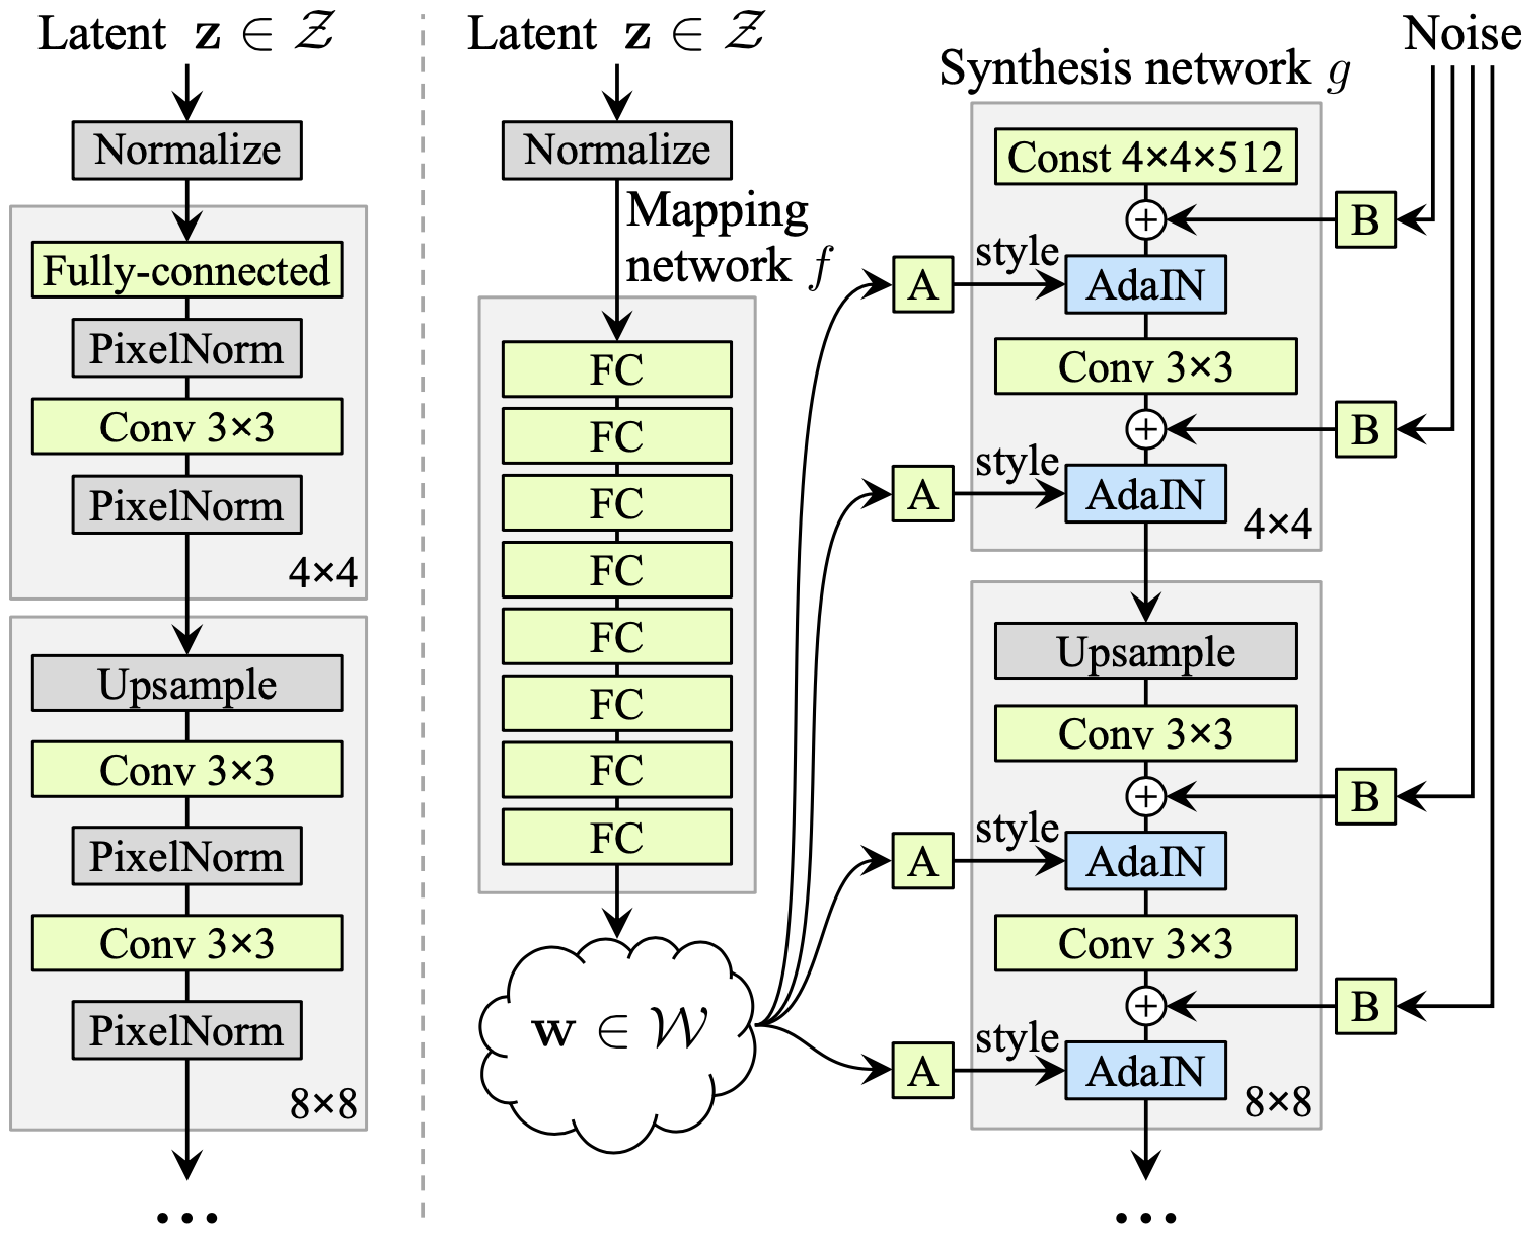
\includegraphics[width=290pt]{figures/figure_11.pdf}
\caption{Style\ac{GAN} architecture \cite{stylegan}. On the left, we have the Prog\ac{GAN} architecture, while on the right we have the proposed Style\ac{GAN} version with the mapping network and style injection.}
\label{fig:stylegan}
\end{figure}

After the release of the original Style\ac{GAN}, the same team corrected some of the visual artefacts that it tended to include in the generated images (i.e., "water droplets" and misaligned eyes or teeth). In fact, the "water droplet" effect results from the generator attempting to sneak some information past the normalisation step:

\begin{figure}[h]
\centering
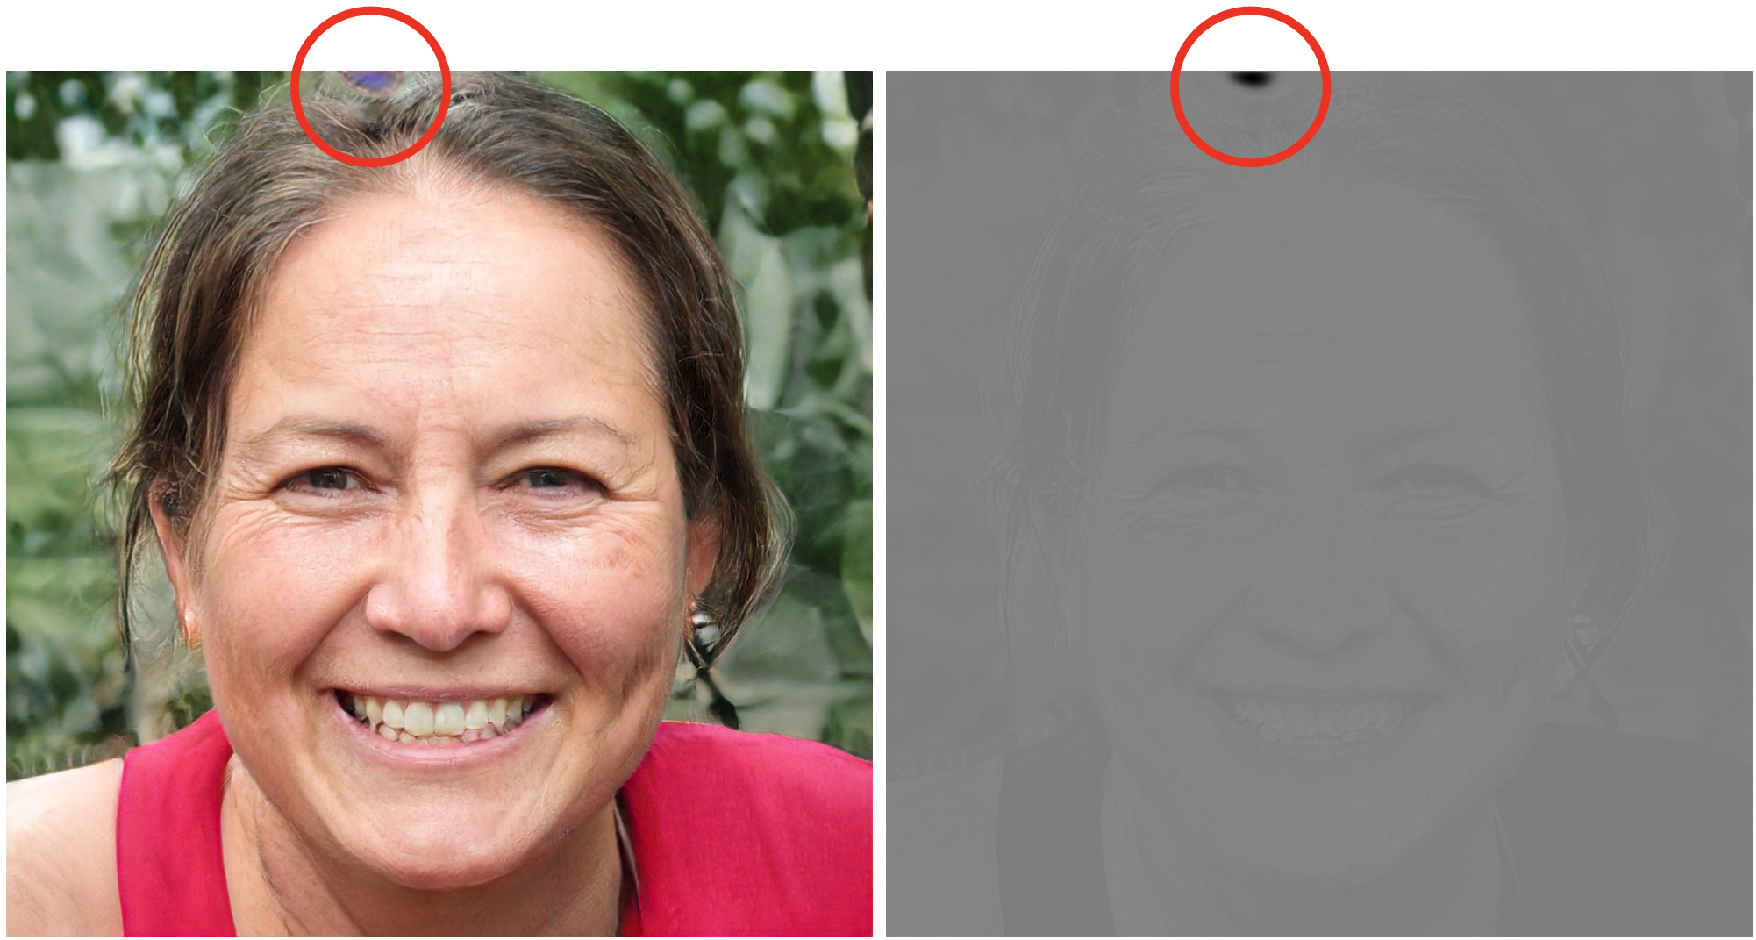
\includegraphics[width=300pt]{figures/figure_12.pdf}
\caption{Water droplet effect generated by the original Style\ac{GAN} design \cite{stylegan}.}
\label{fig:stylegan}
\end{figure}

The Style\ac{GAN}$2$ framework \cite{stylegan2}, as it ended up being called, redesigned the way style vectors are incorporated into the generation process, due to a belief that the \ac{AdaIN} operation limited the generator's ability to use the maximum amount of information. Furthermore, the revised architecture replaced progressive growing with input/output skip connections (for the generator) and residual connections (for the discriminator):\\

\begin{figure}[h]
\centering
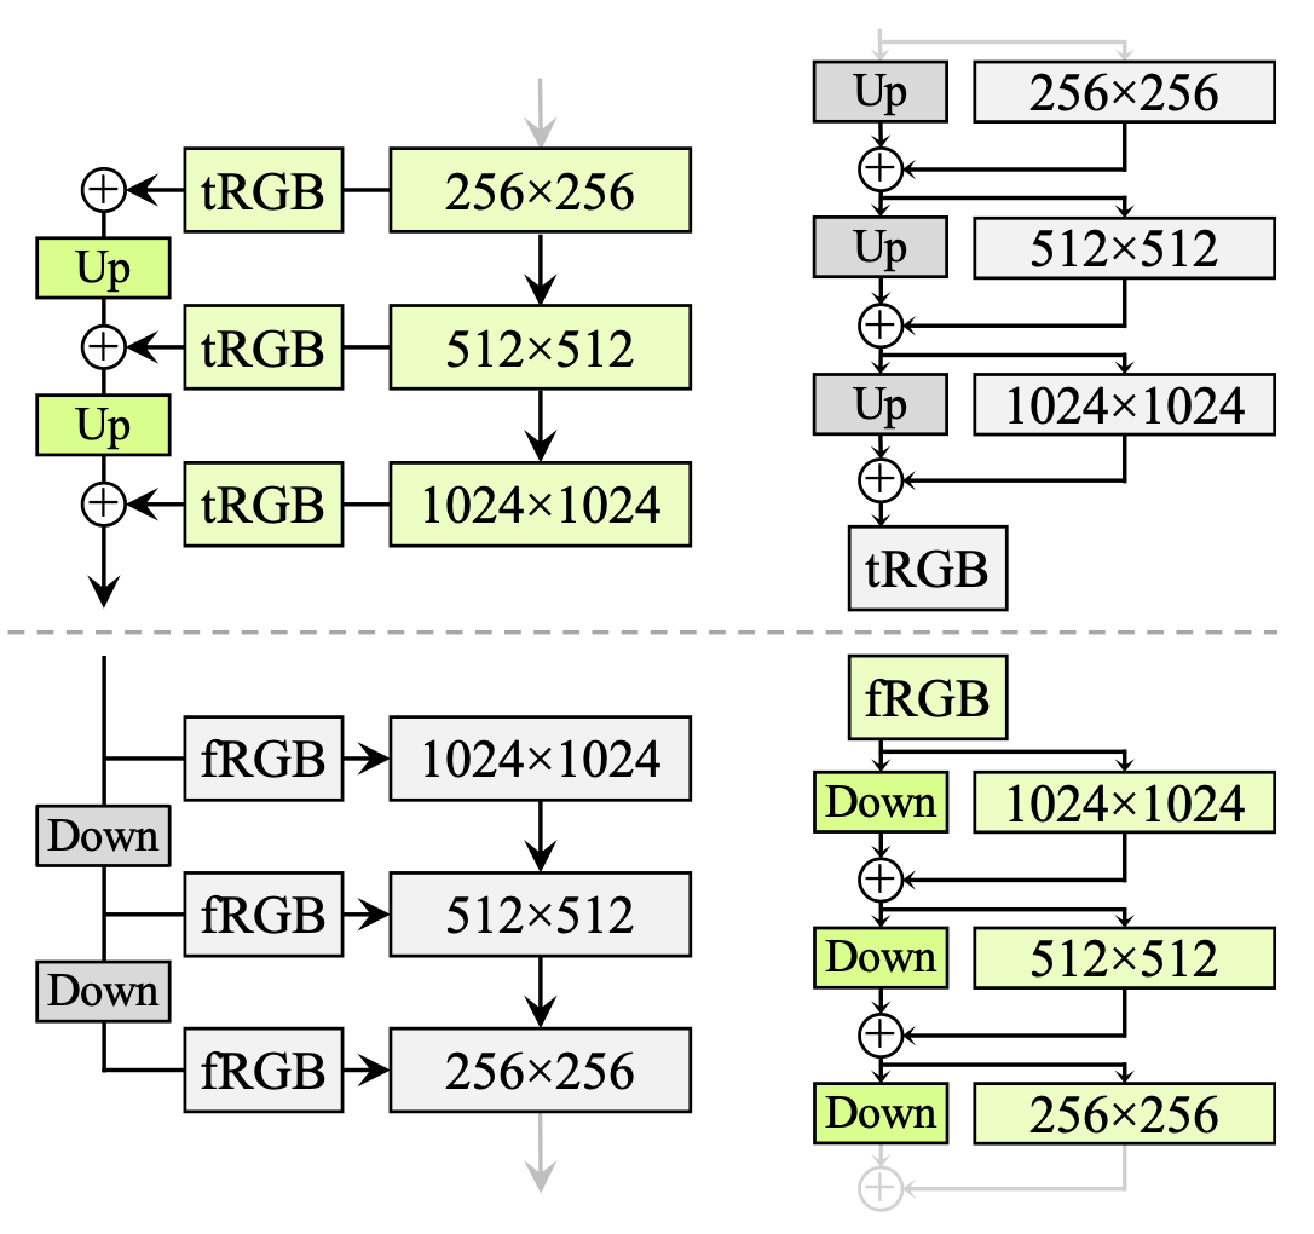
\includegraphics[width=230pt]{figures/figure_13.pdf}
\caption{Proposed revisions of the networks' architectures \cite{stylegan2}. On the left, we have input/output skip connections and, on the right, residual style connections. After some experiments, the authors settled on a skip generator (top-left) combined with a residual discriminator (bottom-right).}
\label{fig:stylegan_2}
\end{figure}

The improved architecture allowed both networks to have access to every resolution layer from the beginning, but only make use of them if it proved beneficial during training. This revision, along with several others, improved what was already a state-of-the-art design, elevating the quality of synthetic imagery even further.

\subsection{Long Short Term Memory}
\label{subsec:chap2_lstm}
As seen before, many \ac{DL} architectures are particularly tuned for problems like image classification or synthesis. However, in other tasks, such as text generation, a model must be able to retain some of the information received previously. This notion of context is particularly addressed by a family of models known as \ac{RNN}s. They comprise loops that feed the output back to the unit, allowing it to combine both new and previous information.

\begin{figure}[h]
\centering
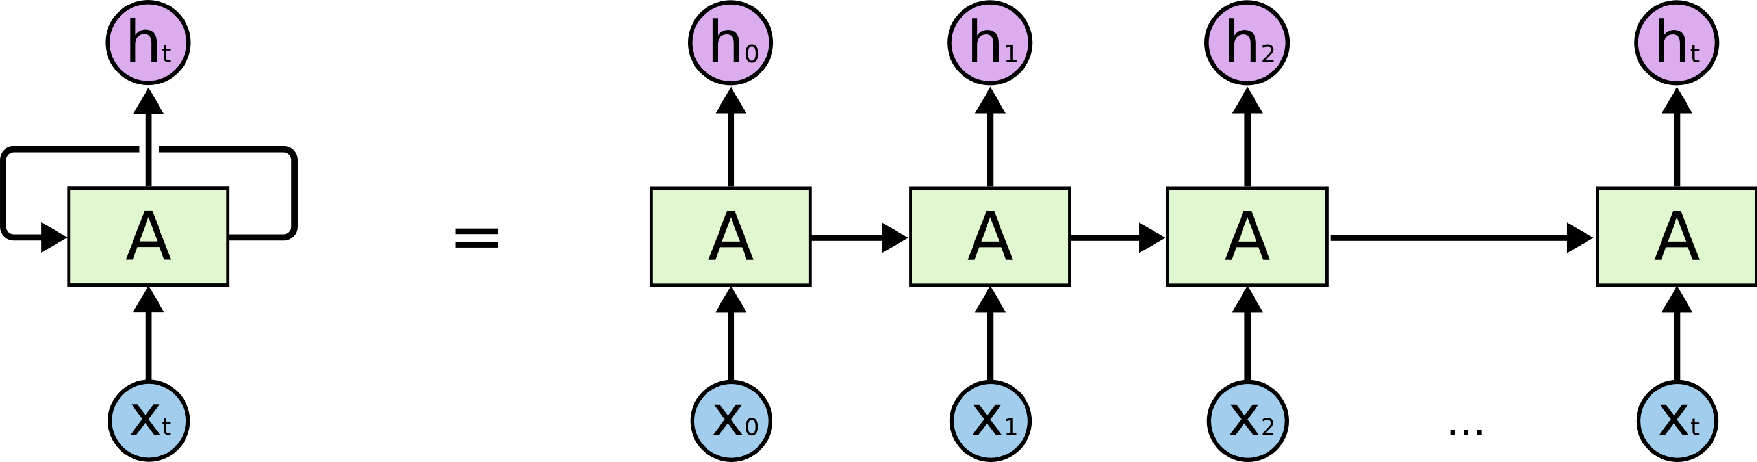
\includegraphics[width=330pt]{figures/figure_14.pdf}
\caption{Visualisation of a single unit from a \ac{RNN} \cite{lstm_explained}. On the left, the unit is seen as theory describes it, while on the right, the loop is expanded indefinitely to form a chain (for explaining purposes).}
\label{fig:rnn_unit}
\end{figure}

An architecture similar to the above is perfectly suited for dealing with sequences and lists. Considering their applicability to text generation, these networks can infer the likelihood of outputting a word based on the immediately preceding words. For example, in the sentence "The Eiffel Tower is in ..." the most likely word to appear next is "Paris". The gap between the relevant context and where the word needs to appear is quite small. But considering an example like "I have been in France for two years and I love speaking ...", we can realise how much more persistence is needed for the notion of "France" to influence the word that we expect to see at the end (i.e., "French"). To deal with longer-lasting dependencies, a more powerful version of \ac{RNN}s was introduced in the form of \ac{LSTM}s:

\begin{figure}[h]
\centering
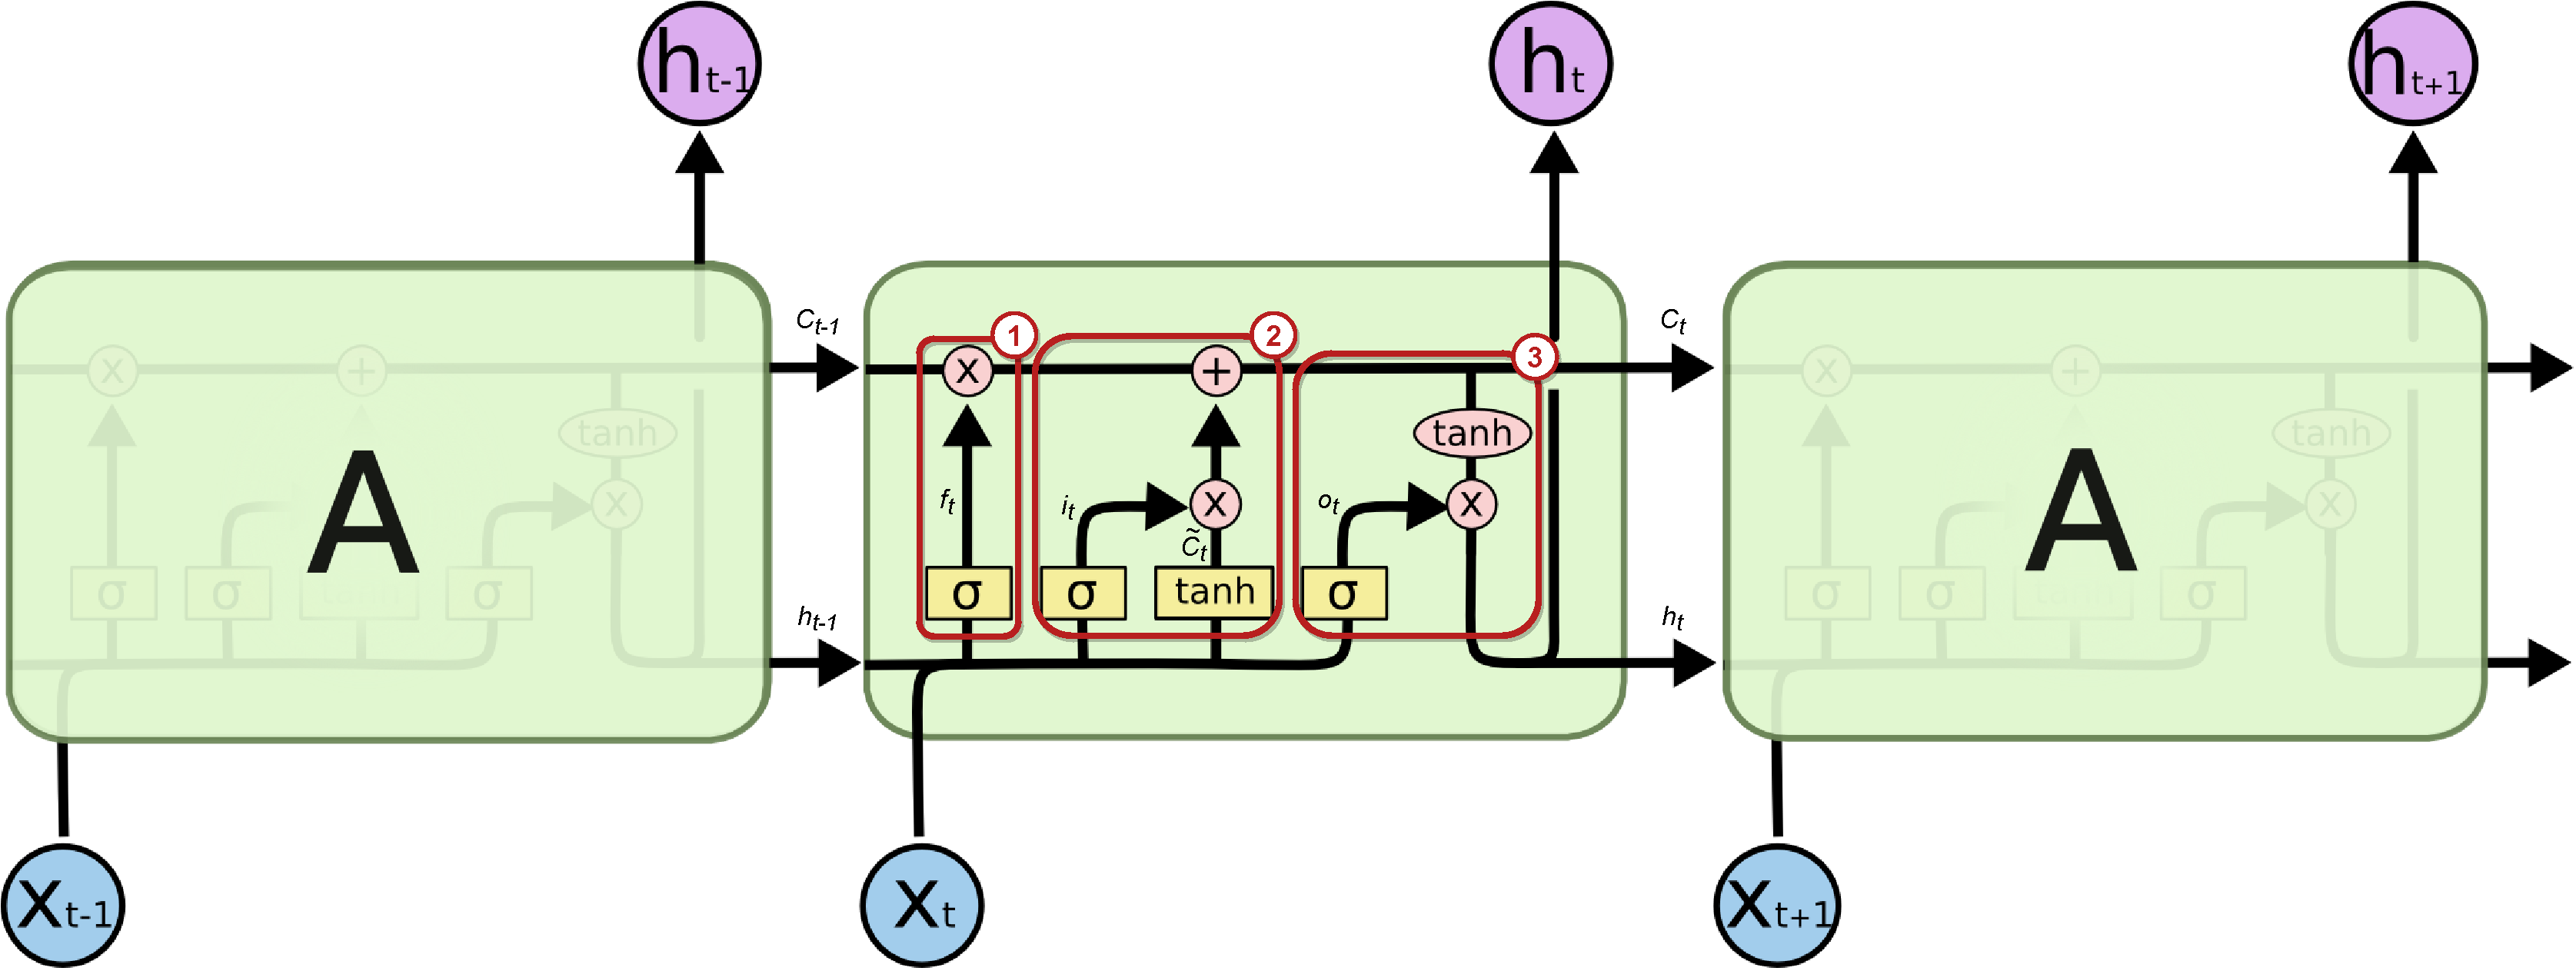
\includegraphics[width=330pt]{figures/figure_15.pdf}
\caption{Representation of an \ac{LSTM}'s inner workings (edited for explaining purposes) \cite{lstm_explained}. The top pathway represents the accumulated context (or cell state), which will be subjected to changes if it proves beneficial. In the lower portion of the schematics, two main steps are responsible for filtering and updating the cell state, based on the new information that the unit receives. Finally, the output is a combination of both the updated context and the new, short-term information.}
\label{fig:lstm_unit}
\end{figure}

More formally, the top pathway (commonly described as the cell state) represents the previously discussed notion of context (i.e., what we know so far). It is updated in steps $1$ and $2$, by filtering and adding information, respectively.\\

As an input $x_{t}$ enters the unit (step $1$), it is added to the output of the previous unit ($h_{t-1}$) and weighted by the learned weights. Then, the sigmoid function takes that summation and maps it to a value ranging from $0$ to $1$. It is this value $f_{t}$ that, when multiplied by the current cell state $C_{t-1}$, determines if the context is to be forgotten or kept. These gates, as they are also called, allow the \ac{LSTM} to have more control and sensibility.

Next (step $2$), having a filtered context, we must determine how much new information should be added to that context. To do so, a weighted summation of $h_{t-1}$ and $x_{t}$ is once again given to a sigmoid function which creates a filter (just like before). Parallel to this computation, $h_{t-1}$ and $x_{t}$ are given to a tanh function which maps them to a value from $-1$ to $1$, later multiplied by the filter. The resulting value is then added to the filtered context, thus creating a newly updated context (or cell state).

Finally, the output of the unit is comprised of the updated cell state conditioned on the new information $h_{t-1}$ and $x_{t}$: the tanh function maps the updated context to a value from $-1$ to $1$, later multiplied by the filter derived from the application of sigmoid to the weighted summation between $h_{t-1}$ and $x_{t}$.\\

Upon closer inspection, it becomes clear how the \ac{LSTM} unit performs as expected: steps $1$ and $2$ update the knowledge gathered so far, based on the new information received, and then step $3$ focuses on outputting a value that is not only based on the short-term information (that is what $h_{t-1}$ and $x_{t}$ represent) but also on the new long-term context.

\section{Machine Learning Explainability}
\label{sec:chap2_machine_learning_explainability}

As an example of what this topic is all about, let us imagine a binary classifier whose task would be to distinguish between wolves and huskies \cite{molnar2019}. After training, it ends up misclassifying a number of huskies as wolves. Explainability techniques could, perhaps, show a tendency for the classifier to use snow, in some of the images, as a feature for the class "wolf". Without these techniques, it would be decidedly harder to reach the same conclusion. Thus, the adoption of a higher degree of transparency can bridge the gap between humans and \ac{ML} models, increasing the level of trust between the two parties.\\

In \cite{mythos_of_model_interpretability}, the author highlights the different degrees of explainability in \ac{ML} models. We might link the word "explainable" to the model's architecture, meaning that it can be easily understood, even if that simple nature leads to a deficiency in capacity. We might also consider the model's parameters as an explainable component. There seem to be many possible (and equally valid) forms of explainability. Therefore, authors in this field have debated on the most accurate taxonomy to describe the scope and depth of what it means to be an explainable system.\\

The proposed criteria \cite{molnar2019, mythos_of_model_interpretability} classifies \ac{ML} Explainability in terms of depth, scope and model applicability:

\begin{itemize}
    \item \textbf{Intrinsic or Post hoc}: are we reducing the model's complexity to make it more explainable? Or are we allowing the model to be complex and only explaining its output?
    \item \textbf{Local or Global}: are we explaining individual predictions? Or the behaviour of the entire model?
    \item \textbf{Model-specific or Model-agnostic}: are the techniques specific to a limited range of models (i.e., only work with them)? Or are they generic enough to be paired with practically any kind of \ac{ML} model?
\end{itemize}

Following the above criteria, we argue that our approaches (chapter \ref{chap3:proposed_methods}) are Post hoc, Local and Model-agnostic. In other words, they allow model complexity, explain single instances of data and can be paired with several types of \ac{ML} and/or \ac{DL} models (in specific, different types of classifiers, generative models and instance segmentation architectures).\\

As a natural extension to this introduction, the next subsections attempt to showcase the most common techniques found in the literature. These techniques have ranging levels of complexity and applicability to the problem of periocular recognition. Some of them rely on images, while other make use of plots. Nevertheless, they share a common goal: remove the mist that conceals the reasoning of complex \ac{ML} models. 

\subsection{Partial Dependence Plot}
\label{subsec:chap2_partial_dependence_plot}
A \ac{PDP} is, as the name suggests, a plot relating one or two features with a target variable \cite{pdp}. Ideally, the features have to be independent in order to properly explain the behaviour of another, dependent variable (i.e., target). The main purpose of such technique is to determine the nature of feature-target relationships (e.g., linear or more complex). Additionally, \ac{PDP} is a global explainability method, meaning that it can capture the behaviour of the entire dataset to produce a global relationship between features and targets.

From this point forward (including subsection \ref{subsec:chap2_accumulated_local_effects}), the features we want to explain will be represented by $\mathbf{x}_{S}$ and the remaining ones by $\mathbf{x}_{C}$.\\

As an example, let us consider a simple, linear regression model. In this setting, the Partial Dependence Function, that would allow us to create a plot, has the form:
\begin{equation}
    \hat{f}_{\mathbf{x}_{S}}(\mathbf{x}_{S}) = \int_{\mathbf{x}_{C}}^{}
    f(\mathbf{x}_{S},\mathbf{x}_{C}) \Prob (\mathbf{x}_{C}) d \mathbf{x}_{C}
    \label{eq:3}
\end{equation}
The formulation above shows that the \ac{PDP} values for the features in $\mathbf{x}_{S}$ are the result of marginalising the model $f$ over the distribution of the features present in $\mathbf{x}_{C}$. By doing so, a new model $\hat{f}$ is obtained, depending exclusively on the features in $\mathbf{x}_{S}$. To approximate the indefinite integral, one can take a Monte Carlo approach and average the prediction of instances in the training set (with length $m$), while fixating the values of $\mathbf{x}_{S}$:
\begin{equation}
    \hat{f}_{\mathbf{x}_{S}}(\mathbf{x}_{S}) = \frac{1}{m} \sum^{m}_{i=1}f(\mathbf{x}_{S},\mathbf{x}_{C}^{(i)})
    \label{eq:4}
\end{equation}
It becomes evident, then, that the basic principle of \ac{PDP} is the lack of correlation between the features in $\mathbf{x}_{S}$ and the ones in $\mathbf{x}_{C}$, which is usually not the case.

Suppose we only have weight ($\mathbf{x}_{S}$) and height ($\mathbf{x}_{C}$) as features. If a given value of $\mathbf{x}_{S}$ is fixated, all the other possible values for $\mathbf{x}_{C}$, observed in the training data, will be paired with that specific value of $\mathbf{x}_{S}$. In many cases, unlikely combinations will appear, like an instance where a really small weight will be paired with a really high height. It simply comes down to the fact that these two features are heavily dependent on each other. Unfortunately, such limitation limits \ac{PDP}'s applicability in a plethora of cases.\\

In spite of this, in situations where the chosen features are independent, this technique can even be used for classification problems, in which case the \ac{ML} model outputs class probabilities. Consequently, a \ac{PDP} would display the class, as the dependent variable, and one or two features as the independent ones. To get a broader perspective, one could simply create a \ac{PDP} per class.\\

To better understand and visualise this concept, Fig. \ref{fig:partial_dependence_plot} shows three different variables (features) being individually plotted against the target variable (in this case, the number of bike rentals on any given day). Note that here we are using the model $\hat{f}$, which only requires one input variable at a time, given that the remaining variables were marginalised:

\begin{figure}[h]
\centering
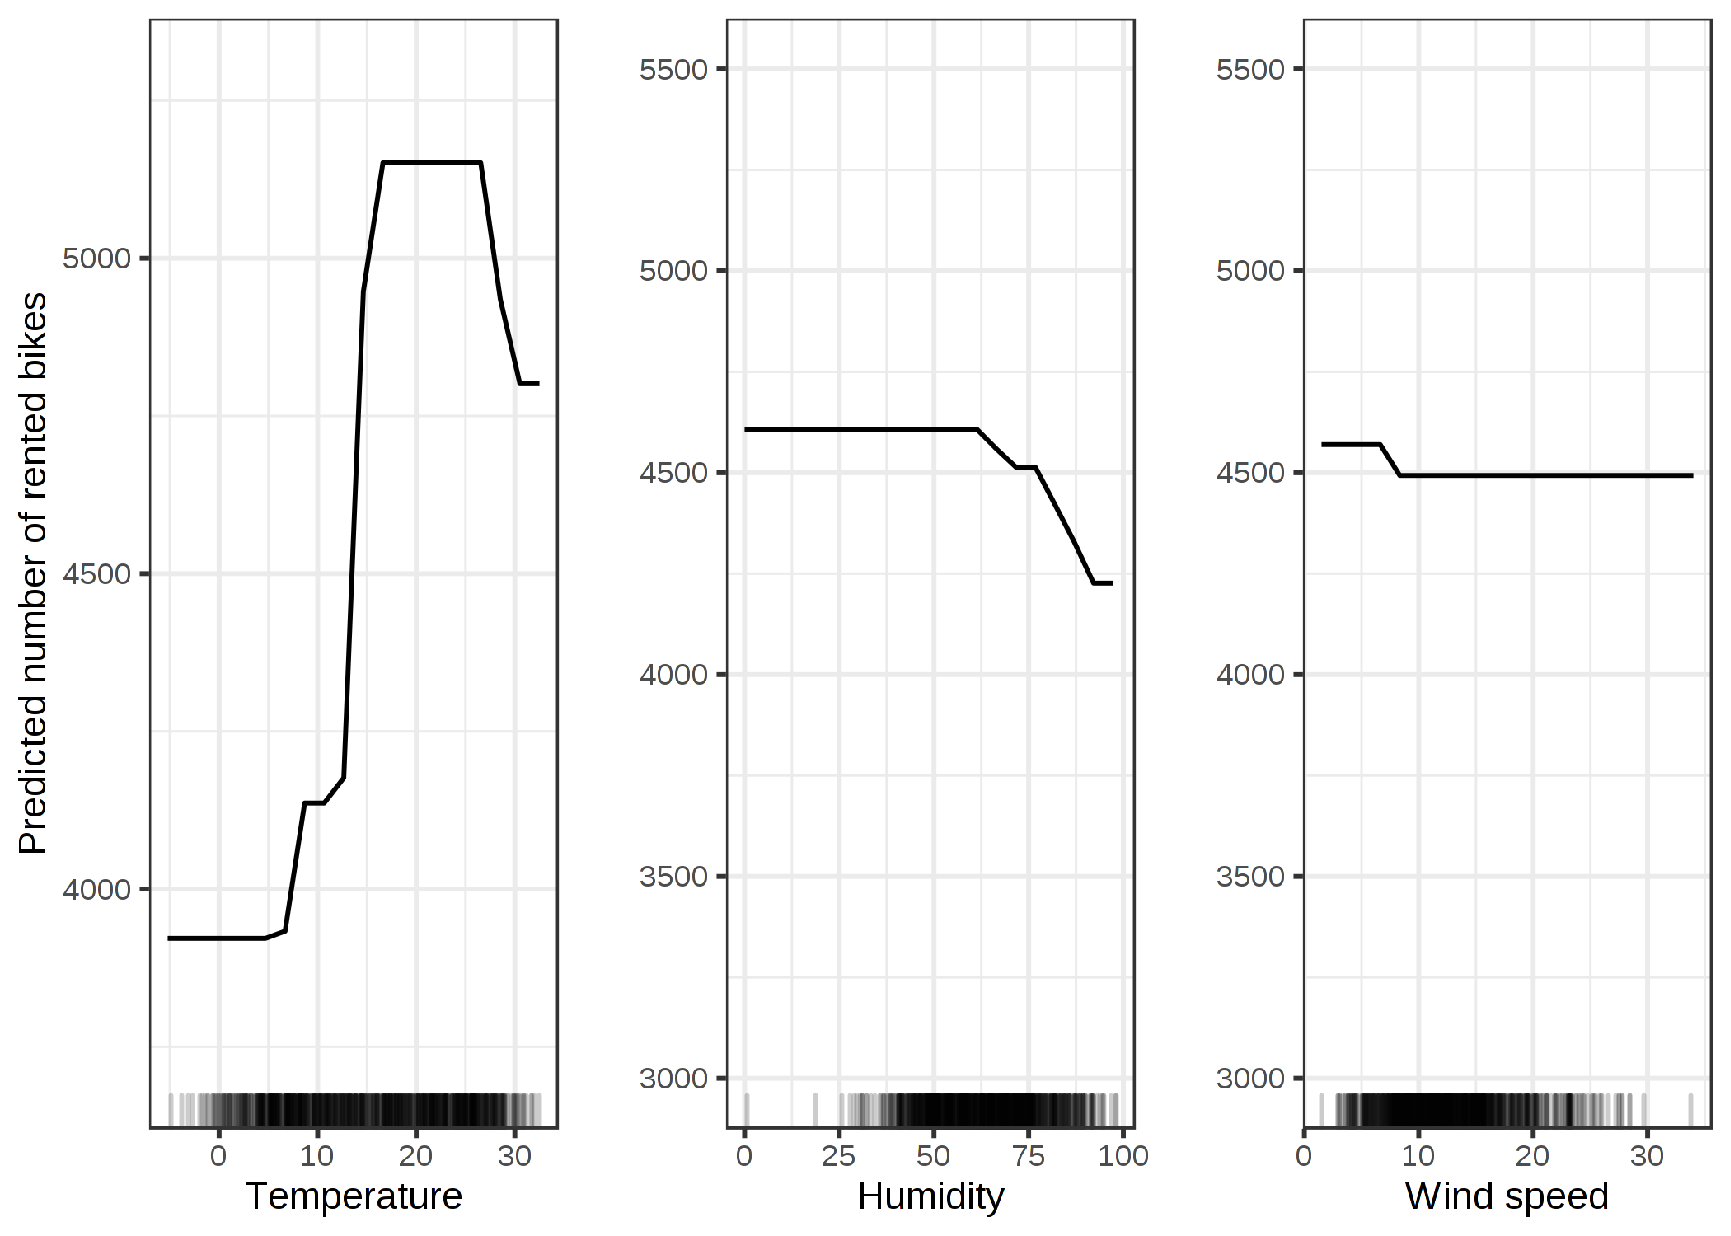
\includegraphics[width=245pt]{figures/figure_16.pdf}
\caption{Three \ac{PDP}s from a regression model with three independent variables and one, dependent variable \cite{molnar2019}. The predicted values come from a marginalised model ($\hat{f}$) that only relies on one feature.}
\label{fig:partial_dependence_plot}
\end{figure}

As an explainable technique, \ac{PDP} works well if its conditions are met (variable independence and need for only one or two features per plot).
However, when features become too entangled, \ac{PDP} can produce unreliable results \cite{molnar2019}.\\

Considering the purposes of this work, this method will not suffice for two main reasons. Firstly, our attributes are, intuitively, entangled: blue-eyed people tend to have lighter skin tones, as opposed to darker skin tones, which often accompany darker iris shades. Feature independence is much more theoretical and usually present in toy problems.  Secondly, it is simply not enough to display just one or two features at a time.

\subsection{Accumulated Local Effects}
\label{subsec:chap2_accumulated_local_effects}

Another technique that produces plots is \ac{ALE}, commonly cited as an alternative to \ac{PDP}, particularly due to the latter's unreliability when the features are correlated \cite{ale}.

Before getting into the formulas, it is important to visualise \ac{ALE}'s reasoning:

\begin{figure}[h]
\centering
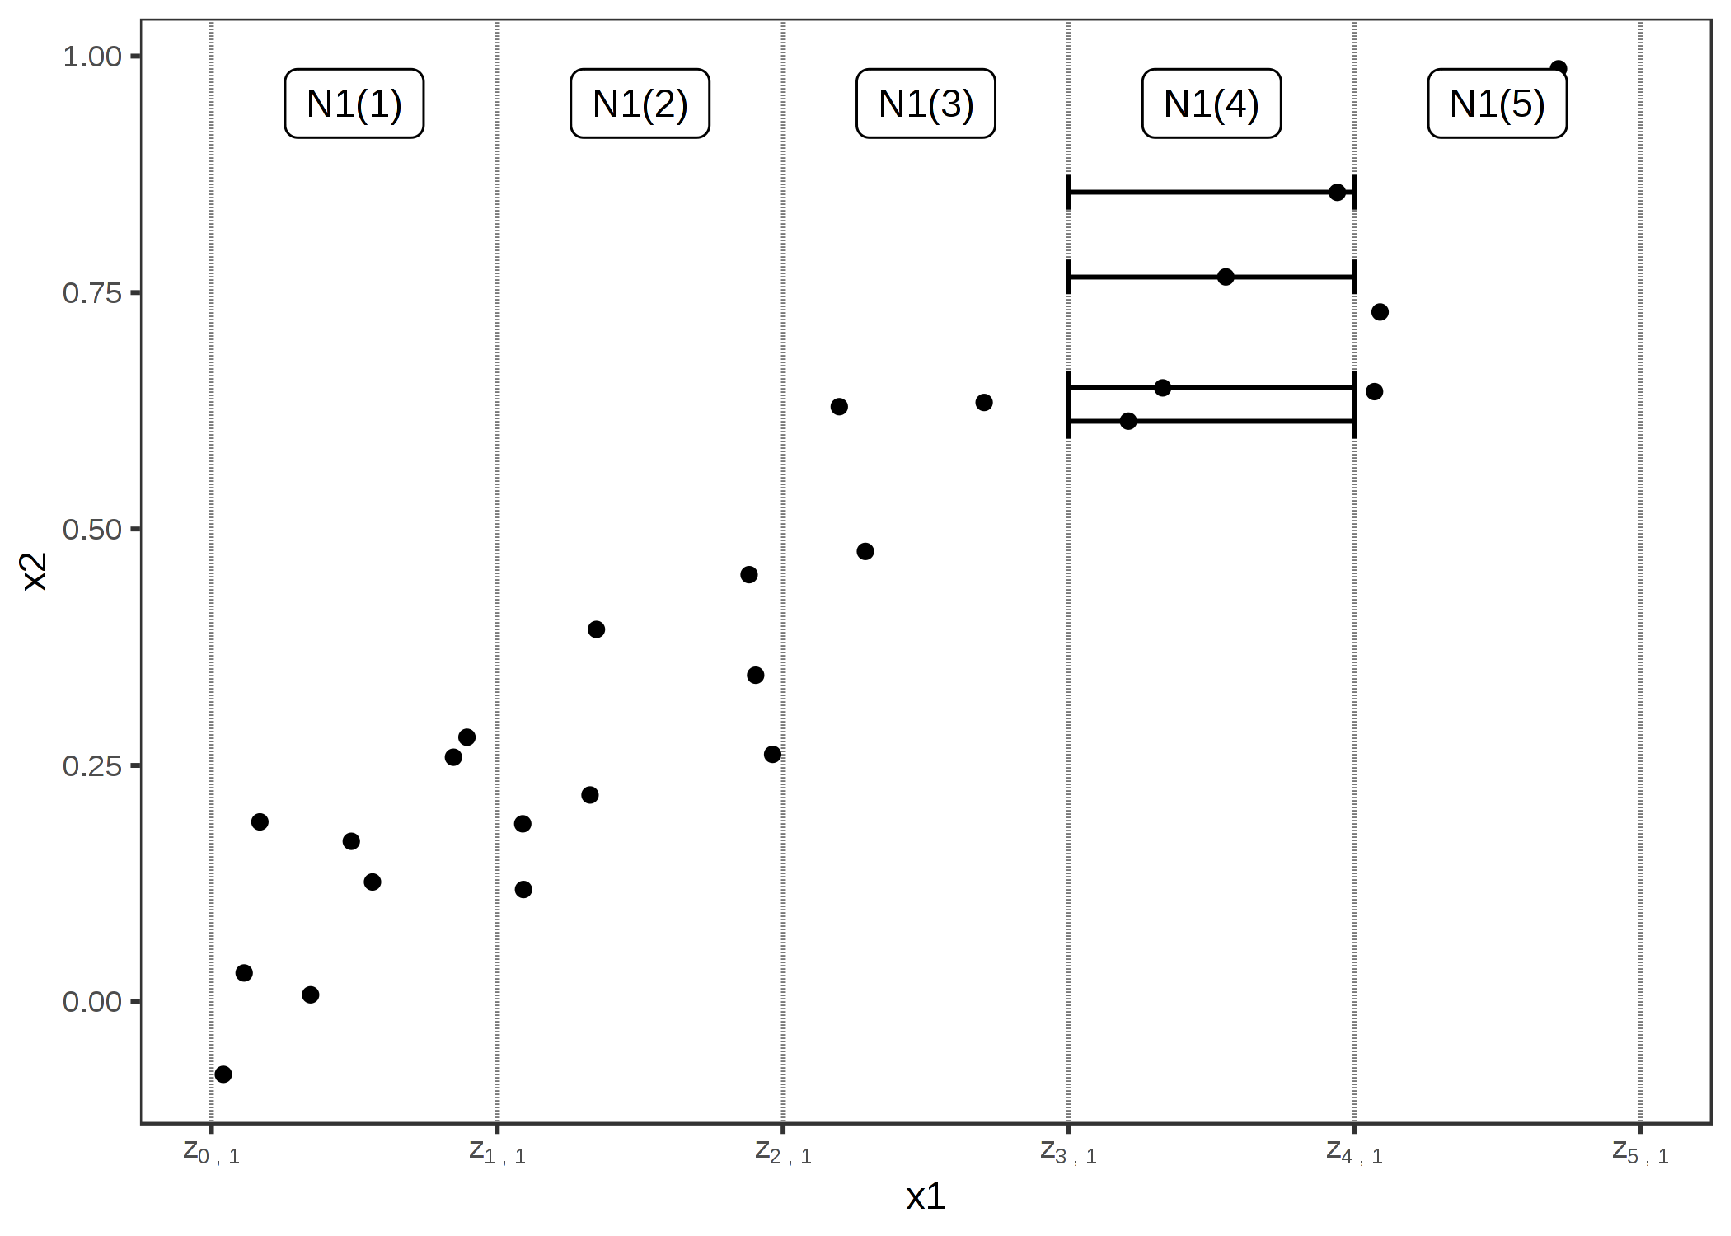
\includegraphics[width=245pt]{figures/figure_17.pdf}
\caption{Calculation of \ac{ALE} for feature $\mathbf{x}_1$, strongly correlated with feature $\mathbf{x}_2$ \cite{molnar2019}. The distribution in divided into intervals and, for each one, we determine the difference in predictions when feature $\mathbf{x}_1$ takes on the values of the lower and upper limits. These results are later accumulated (i.e., summed) and centred.}
\label{fig:accumulated_local_effects_grid}
\end{figure}

From the figure above, we get the idea that \ac{ALE} evaluates differences in predictions at a smaller scale (i.e., the intervals) and then sums everything to get a broader perspective on how the model $f$ behaves. Indeed, that is what the next formula describes:
\begin{equation}
    \hat{f}_{\mathbf{x}_{S}}(\mathbf{x}_{S}) = \int_{\mathbf{z}_{0,1}}^{\mathbf{x}_{S}} \int_{\mathbf{x}_{C}}^{} \frac{\partial f(\mathbf{z}_{S},\mathbf{x}_{C})}{\partial \mathbf{z}_{S}} \Prob (\mathbf{x}_{C}|\mathbf{z}_{S}) d \mathbf{x}_{C} d \mathbf{z}_{C} - c
    \label{eq:7}
\end{equation}

In equation \ref{eq:7}, \ac{ALE} also tries to produce a new model that only requires the features in $\mathbf{x}_{S}$. The difference with regards to \ac{PDP} comes from the fact that we do not use all the possible values for the features in $\mathbf{x}_{C}$, but rather, the values that are possible in the range that our specific feature values belong to ($ \Prob (\mathbf{x}_{C}|\mathbf{z}_{S})$). By using a conditional distribution, we eliminate the unlikely combinations that \ac{PDP} would have considered. Then, the leftmost integral applies the same reasoning to the entire range of possible values for the features that $\mathbf{x}_{S}$ contains. Finally, a constant $c$ is subtracted to ensure that, in the \ac{ALE} plot, the average effect is zero. \\

As an example, the next couple of formulas are going to describe how the \ac{ALE} values are calculated when we want to use just one feature (this method is broad enough to work for two features at a time and even for categorical features).

Just like with \ac{PDP}, in practice we approximate the theoretical definition, and, in this case, that process is done with the following formula:
\begin{equation}
    \hat{f}_{j}(x) = \sum_{k=1}^{k_{j}(x)} \frac{1}{|\mathbf{n}_{j}(k)|} \sum_{i:\mathbf{x}_{j}^{(i)} \in \mathbf{n}_{j}(k)} [f(\mathbf{z}_{k,j},\mathbf{x}_{\setminus j}^{(i)}) - f(\mathbf{z}_{k-1,j},\mathbf{x}_{\setminus j}^{(i)})]
    \label{eq:8}
\end{equation}

Starting from the right, in $[f(\mathbf{z}_{k,j},\mathbf{x}_{\setminus j}^{(i)}) - f(\mathbf{z}_{k-1,j},\mathbf{x}_{\setminus j}^{(i)})]$, we are interested in determining the difference in predictions when we replace the value of the feature $j$ we want to explain with the values from the upper ($\mathbf{z}_{k,j}$) and lower ($\mathbf{z}_{k-1,j}$) limits of a given interval. The summation $\sum_{i:\mathbf{x}_{j}^{(i)} \in \mathbf{n}_{j}(k)}$ allows us to repeat the aforementioned process for every instance whose feature $j$ belongs to a neighbourhood given by $\mathbf{n}_{j}(k)$. If we recall Fig. \ref{fig:accumulated_local_effects_grid}, these neighbourhoods are the vertical slices that divide feature $j$'s distribution. Then, to average the differences we divide the summation by the number of instances in the given interval ($|\mathbf{n}_{j}(k)|$). This part of the formula computes the local effect of feature $j$.

Following the above steps, the leftmost summation is responsible for computing and, more importantly, accumulating the local effects of every interval (thus giving meaning to the acronym \ac{ALE}). Finally, we subtract the average to the resulting values, ensuring that they stay centred around zero:
\begin{equation}
    \hat{f}_{j}(\mathbf{x}_j) = \hat{f}_{j}(\mathbf{x}_j) - \frac{1}{m} \sum_{i=1}^{m} \hat{f}_{j}(\mathbf{x}_{j}^{(i)})
    \label{eq:9}
\end{equation}

Fig. \ref{fig:accumulated_local_effects} depicts an \ac{ALE} plot of the problem seen in subsection \ref{subsec:chap2_partial_dependence_plot}. This example shows that the plots are indeed centred around zero, with positive values indicating an increase in the model's prediction and negative values indicating a decrease, when compared to the average prediction. Additionally, it becomes clear how shaky \ac{ALE} plots can be, especially when compared with the \ac{PDP} version (as a side note, the number of intervals contributes to this effect):

\begin{figure}[h]
\centering
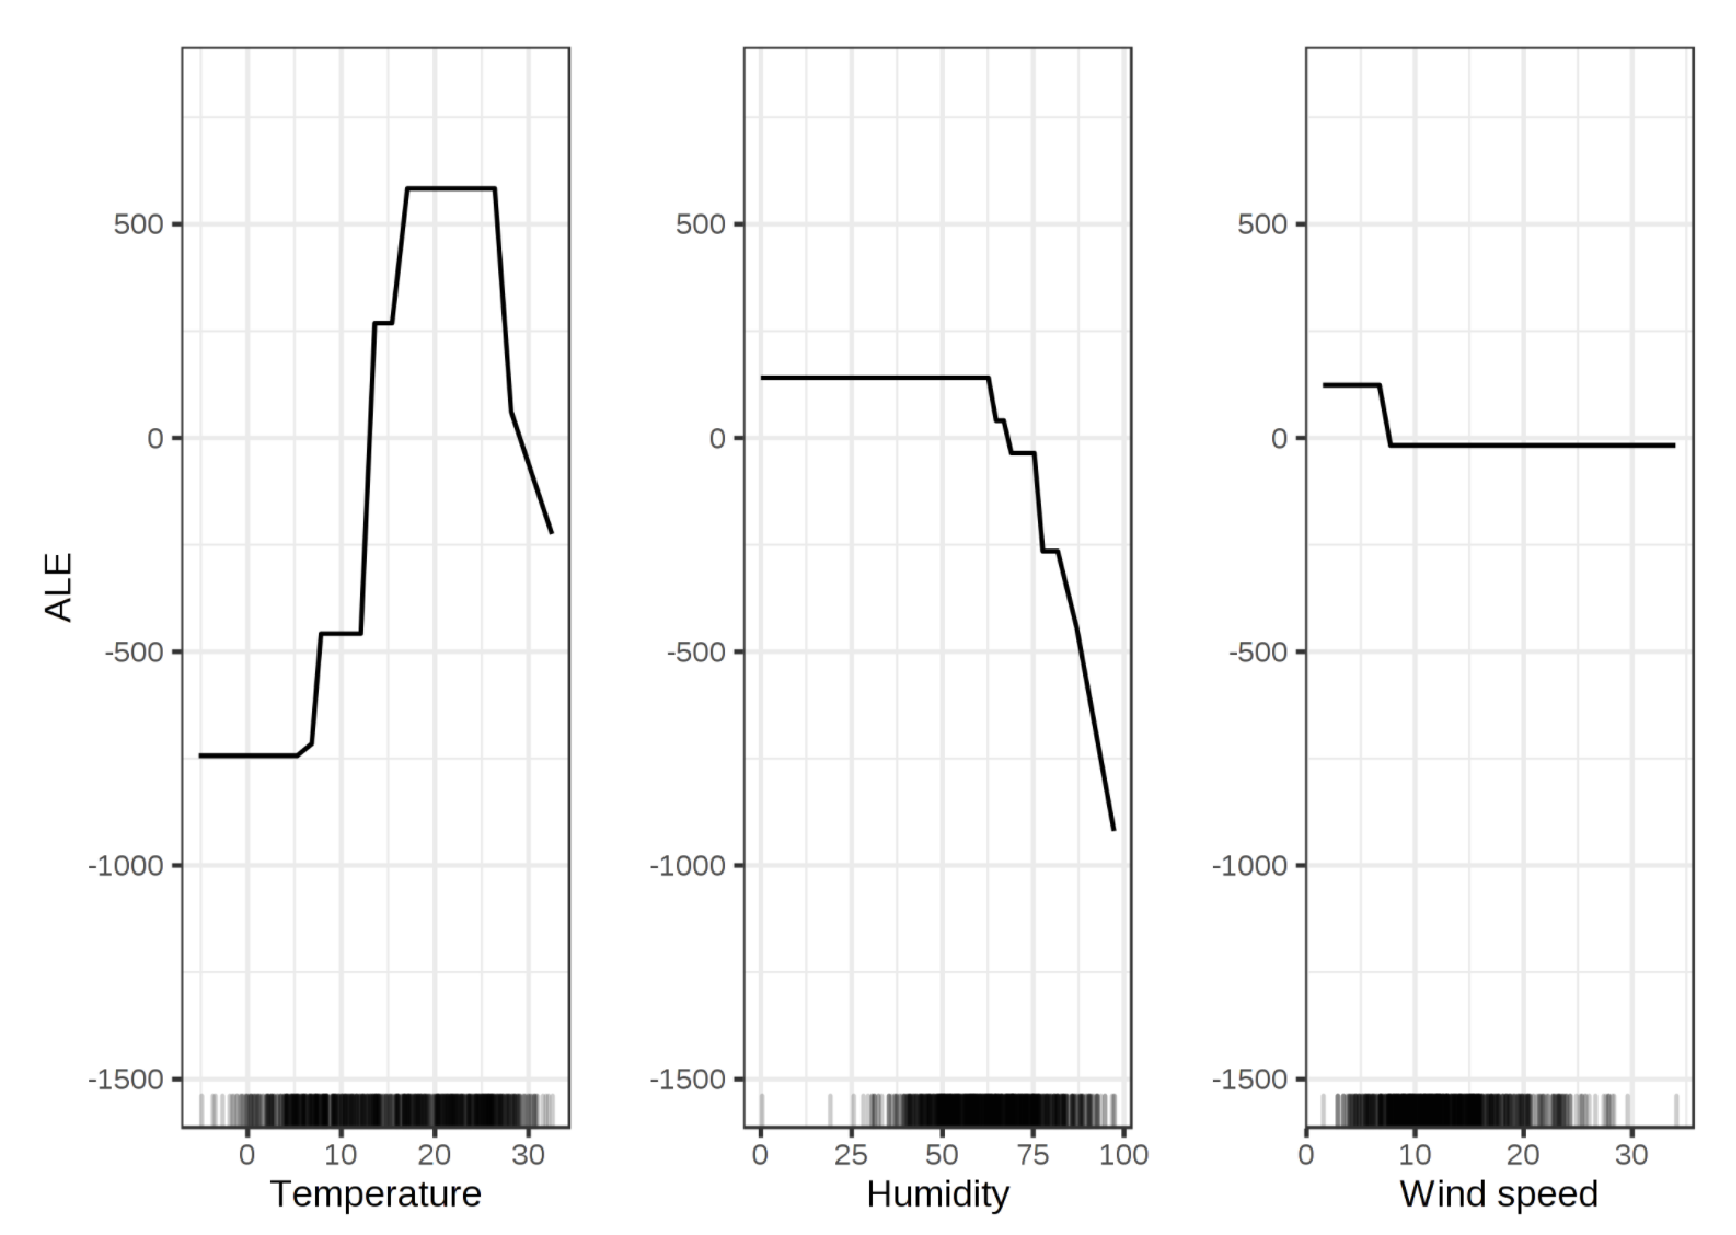
\includegraphics[width=250pt]{figures/figure_18.pdf}
\caption{Three \ac{ALE} plots from a regression model with three independent variables and one, dependent variable \cite{molnar2019}. As per the trained model, the temperature and humidity's influence outweights that of the wind speed.}
\label{fig:accumulated_local_effects}
\end{figure}

Overall, \ac{ALE} plots are considered a superior technique to \ac{PDP}s, despite having some drawbacks too: as mentioned before, the shaky lines can become undesirable and the implementation of this method is more complex. In spite of this, it is generally accepted that, when we are working with independent variables and require fast computing times, \ac{PDP} is the preferred option. For virtually any other scenario, \ac{ALE} is regarded as the superior solution.\\

Just like \ac{PDP}, and despite being better for the specific use case described in the present document, the visualisation of only a couple features limits \ac{ALE}'s applicability. The following subsections will describe other methods that come closer to what is expected from a framework that can, visually, explain its decisions.

\subsection{Occlusion Map}
\label{subsec:chap2_occlusion_map}
Being one of the most straightforward techniques, Occlusion Maps try to make perturbations on certain areas of  an input image and register how the model (usually a classifier, like a \ac{CNN}) reacts to those changes.\\

In practice, this method involves taking a square, of fixed size and colour, and sliding it over the image, iteratively. Then, the perturbed images are fed to the classifier and its scores are noted. Finally, the scores are translated into a heat map, indicating the portions of the image where an occlusion had the most impact (i.e., the areas most used by the model to predict the correct class).\\

Fig. \ref{fig:occlusion_map_1} shows a clear example of what kind of results can be expected with this technique. Another example can be found in \cite{occlusion_maps} and Fig. \ref{fig:occlusion_map_2}, where the authors went even further by visualising feature maps and noticing how the classifier would attribute different (wrong) classes when certain parts of the image get occluded:

\begin{figure}[h]
\centering
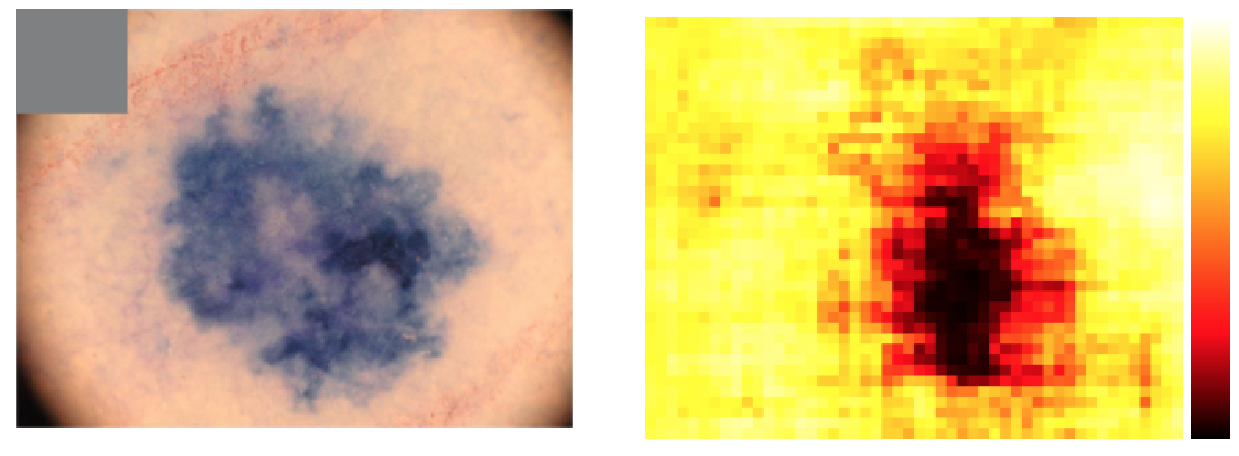
\includegraphics[width=280pt]{figures/figure_19.pdf}
\caption{Example of a heat map generated with the Occlusion Map technique \cite{occlusion_maps_linkedin}. Here, the model clearly identified the melanoma as a crucial element.}
\label{fig:occlusion_map_1}
\end{figure}

\begin{figure}[h]
\centering
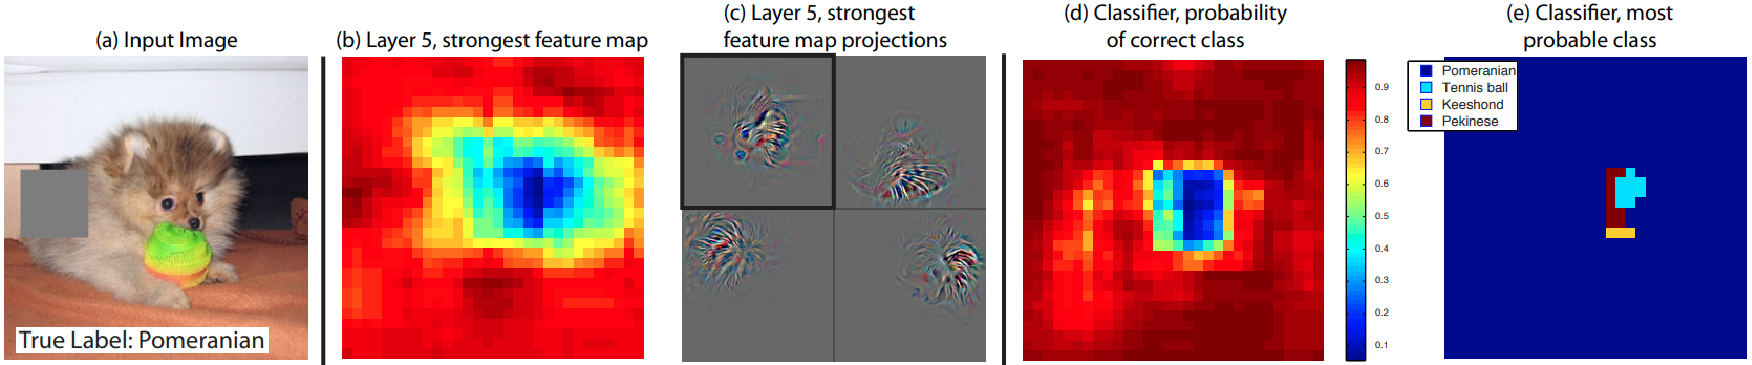
\includegraphics[width=390pt]{figures/figure_20.pdf}
\caption{Another example of Occlusion Maps being used to interpret a model's decisions \cite{occlusion_maps}. The rightmost figure shows how the predicted class varies with respect to occlusions.}
\label{fig:occlusion_map_2}
\end{figure}

As seen above, Occlusion Maps are able to locate areas of an image that contribute the most to a classifier's decision. As an additional benefit, they are also easy to implement and require almost no redesign or retraining of the classifier.\\

The applicability of this technique, however, is somewhat limited, given the need for a higher level explanation (i.e., the ability to highlight well defined areas of the periocular region, like the iris or the eyebrow).

\subsection{Saliency Map}
\label{subsec:chap2_saliency_map}
Described in \cite{saliency_maps}, this technique also attempts to highlight certain parts of the input image with brighter or darker shades, based on their importance to the model's score. The authors propose a simple example to start with, similar to the following:
\begin{equation}
    S_{c}(\mathbf{I}) = \mathbf{w}_{c}^{T} \mathbf{I} + b_{c}
    \label{eq:9}
\end{equation}

Equation \ref{eq:9} comes from a linear score model for class $c$ and, as standard, there is a weight vector $\mathbf{w}_{c}$, which is later transposed, and a bias $b_{c}$. In this setup, each pixel of image $\mathbf{I}$ is weighted according to its importance. 
Translating such formulation to a \ac{CNN} becomes more complicated. In spite of this, one can approximate that value by computing the first-order Taylor expansion:
\begin{equation}
    S_{c}(\mathbf{I}) \approx \mathbf{w}^{T} \mathbf{I} + b
    \label{eq:10}
\end{equation}
In this case, $w$ is the derivative of $S_{c}$ with respect to a specific image $\mathbf{I}_{0}$:
\begin{equation}
    \left. \mathbf{w} = \frac{\partial S_{c}}{\partial \mathbf{I}} \right\rvert_ {\mathbf{I}_{0}}
    \label{eq:11}
\end{equation}
One can interpret equation \ref{eq:11} as obtaining an image-specific class Saliency Map where the magnitude of the derivative indicates the pixels that need to be changed the least to change the final score the most.

Having this foundation, the authors continued the Saliency Map extraction process. Remembering that any image (i.e., $\mathbf{I}_{0}$) has $m$ rows and $n$ columns, a class Saliency Map belongs to $R^{m*n}$. The first step is to find $\mathbf{w}$, as per equation \ref{eq:11} through back-propagation. Then, if $\mathbf{I}_{0}$ is a greyscale image, $\mathbf{w}$ has exactly one element for each pixel, meaning the Saliency Map could be calculated as $\mathbf{M}_{ij} = |\mathbf{w}_{h(i,j)}|$, where $h(i,j)$ is the index of the element in $\mathbf{w}$ directly corresponding to $\mathbf{I}_{0}$'s pixel in row $i$ and column $j$. As for \ac{RGB} images, with multiple depth channels, an index takes the form $h(i,j,c)$ and only the maximum magnitude across all channels is kept: $\mathbf{M}_{ij} = \max_{c}|\mathbf{w}_{h(i,j,c)}|$.

Fig. \ref{fig:saliency_maps} has some examples extracted directly from the original source. It should be note that the three Saliency Maps shown are from the highest scoring class on pseudo-randomly selected \ac{ILSVRC}-$2013$ test images:

\begin{figure}[h]
\centering
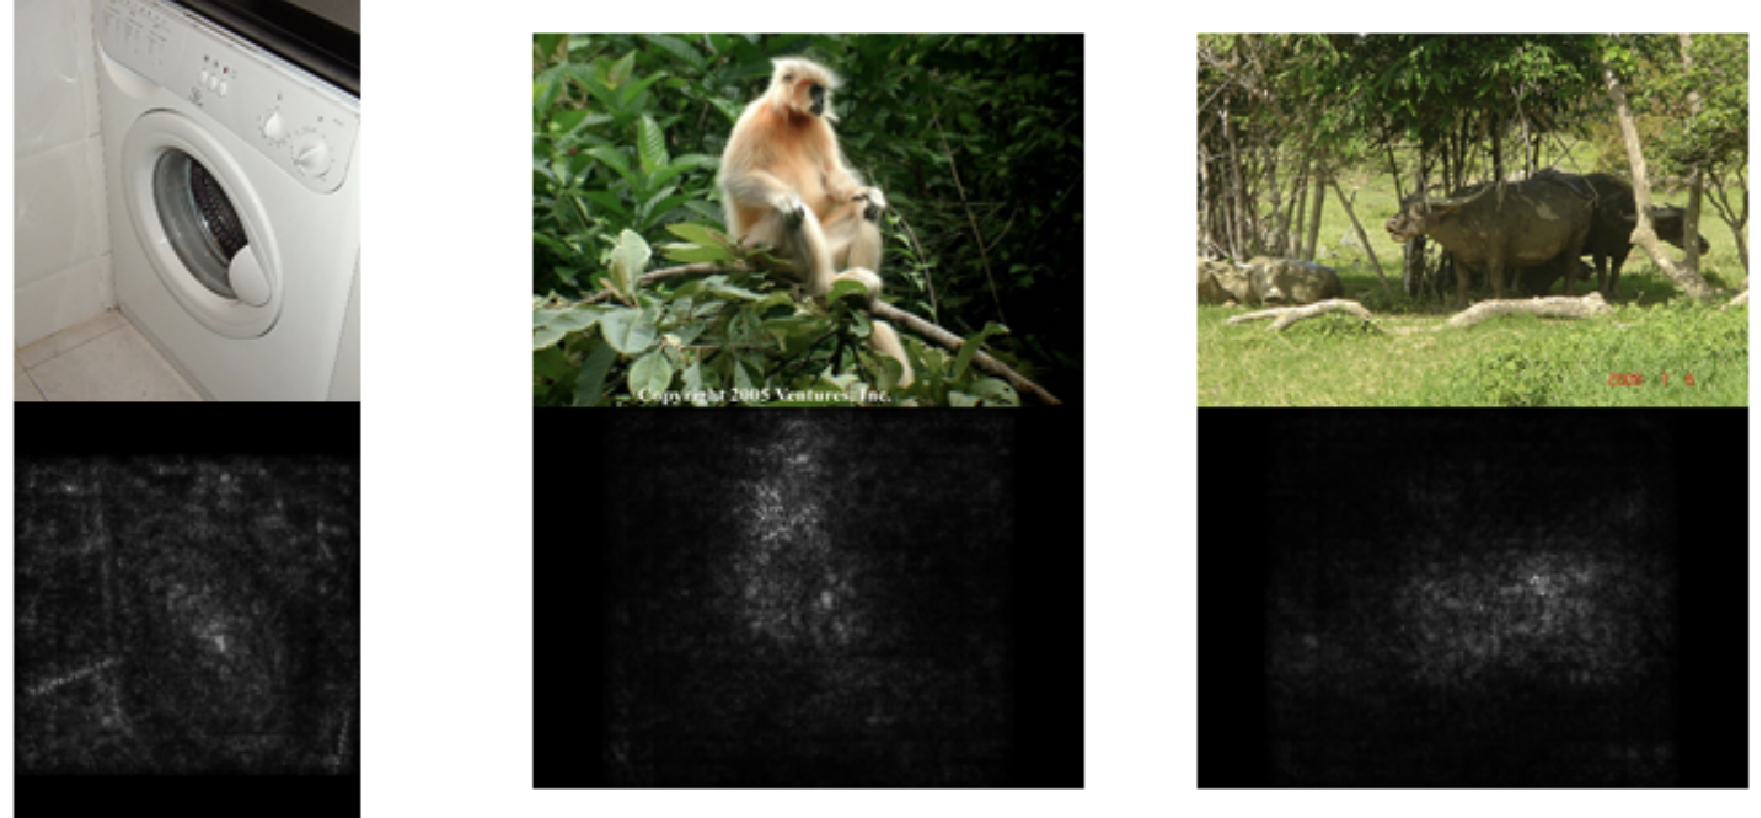
\includegraphics[width=370pt]{figures/figure_21.pdf}
\caption{Three Saliency Maps (below) extracted from each of the input images (above) \cite{saliency_maps}. The pixels in whiter tones are the most significant to the classes that were predicted, meaning that changes to them could impact the output class.}
\label{fig:saliency_maps}
\end{figure}

One advantage of Saliency Maps is that they are not expensive to compute, only requiring a single back-propagation pass, and do not assume the existence of any additional annotations (apart from the labels used when training the original model).\\

The ability to locate the most relevant components of an image fits perfectly into the desirable output of a periocular recognition system (not to mention the higher finesse, when compared with Occlusion Maps). Therefore, subsection \ref{subsec:chap4_explainability_evaluation} presents some results that make use of Saliency Maps to achieve satisfactory levels of explainability.

\subsection{Local Interpretable Model-Agnostic Explanations}
\label{subsec:chap2_local_interpretable_model_agnostic_explanations}
One of the most widely adopted techniques is \ac{LIME}, originally proposed in \cite{lime}. This method relies on surrogate, auxiliary models to, locally, explain the behaviour of a much more complex, black-box model. 

In order to create a basic understanding of how \ac{LIME} works, the authors propose we forget about the training data and assume we only have access to the trained black-box model itself, to which samples can be fed and predictions can be withdrawn. \ac{LIME}'s approach starts by taking a sample and creating variations from it. With this process, a new dataset is created and these samples can be fed to the original, black-box model. Having the dataset and the corresponding predictions, \ac{LIME} moves on to the next phase, where a much simpler model (often linear) is trained with the aforementioned data. The linear model is, however, weighted, meaning that it gives more importance to samples that are closer to the one being explained (thus forcing locality). The learned model should be a good approximation of the original one, albeit locally (the so called local fidelity \cite{molnar2019}).\\

In broader terms, an explanation can be defined 
as follows:
\begin{equation}
    \text{explanation}(x) = \arg \min_{g \in G} L(f,g,\pi_{x}) + \Omega(g)
    \label{eq:12}
\end{equation}
Equation \ref{eq:12} shows how an explanation for an instance $x$ is the summation of a loss component $L$ (e.g., \ac{MSE}) and a complexity component $\Omega$. $L$ measures how the predictions from the surrogate model $g$ and the original model $f$ compare, considering the neighbourhood given by $\pi_{x}$. $\Omega$ controls the degree of complexity of the surrogate model (preferably low). It should be noted that, in practice, \ac{LIME} optimises the former term, with the latter being left to the user's responsibility.\\

One interesting characteristic of this method is that it works for tabular, text or image data. For each of them, \ac{LIME} tries to create the previously mentioned variations by changing certain aspects of the raw data. With tabular data, it varies each feature individually, helped by a normal distribution with mean and standard deviation in accordance to that feature. As for text and images, \ac{LIME} turns words or super-pixels (contiguous patches of neighbouring pixels) on or off. 

Fig. \ref{fig:lime} presents an example on how \ac{LIME} obtains visual explanations:

\begin{figure}[h]
\centering
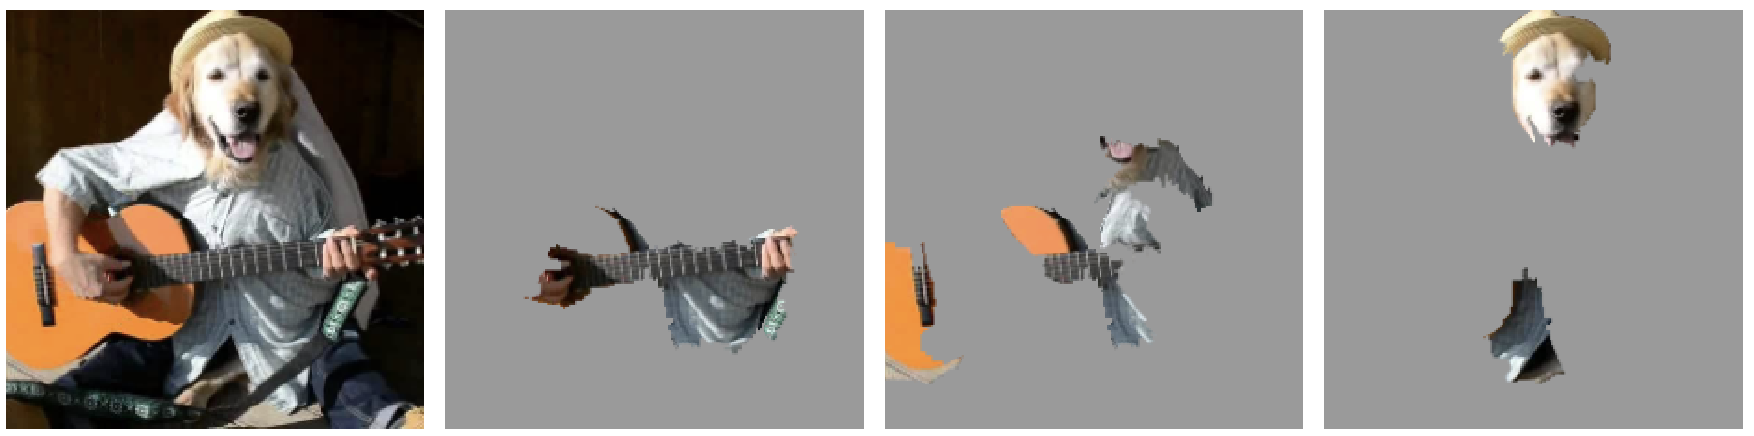
\includegraphics[width=360pt]{figures/figure_22.pdf}
\caption{Inception's top-$3$ predictions ("electric guitar", "acoustic guitar" and "labrador", respectively) explained using \ac{LIME} \cite{lime}. The highest contributing super-pixels were kept, while the remaining ones were greyed out.}
\label{fig:lime}
\end{figure}

\ac{LIME}'s disadvantages include the inherent limitations of linear models, which can be incapable of modelling a complex decision boundary, even if it is local and at a smaller scale. Despite the drawbacks, this technique is certainly capable of providing a hint of explainability to otherwise opaque models. \\

Considering \ac{LIME} is popular and effective, subsection \ref{subsec:chap4_explainability_evaluation} includes a perspective on how it could be applied to the present work.

\subsection{Anchors}
\label{subsec:chap2_anchors}
Following their work with \ac{LIME}, the authors proposed another approach in \cite{anchors}, whose goal is to create decision rules in the form IF-THEN, such that a prediction is sufficiently anchored by some features (i.e., if changes in other feature values do not change the prediction). The techniques employed to that end include reinforcement learning and graph search.\\

Just like \ac{LIME}, this method generates perturbations on real instances to create local explanations. Simple IF-THEN rules are used to explain local behaviours, instead of surrogate models. Additionally, the notion of coverage is introduced to specify the amount of instances a rule applies to (i.e., they are expected to be reusable). Fig. \ref{fig:anchors_1} provides a visualisation of both anchors and \ac{LIME}:

\begin{figure}[H]
\centering
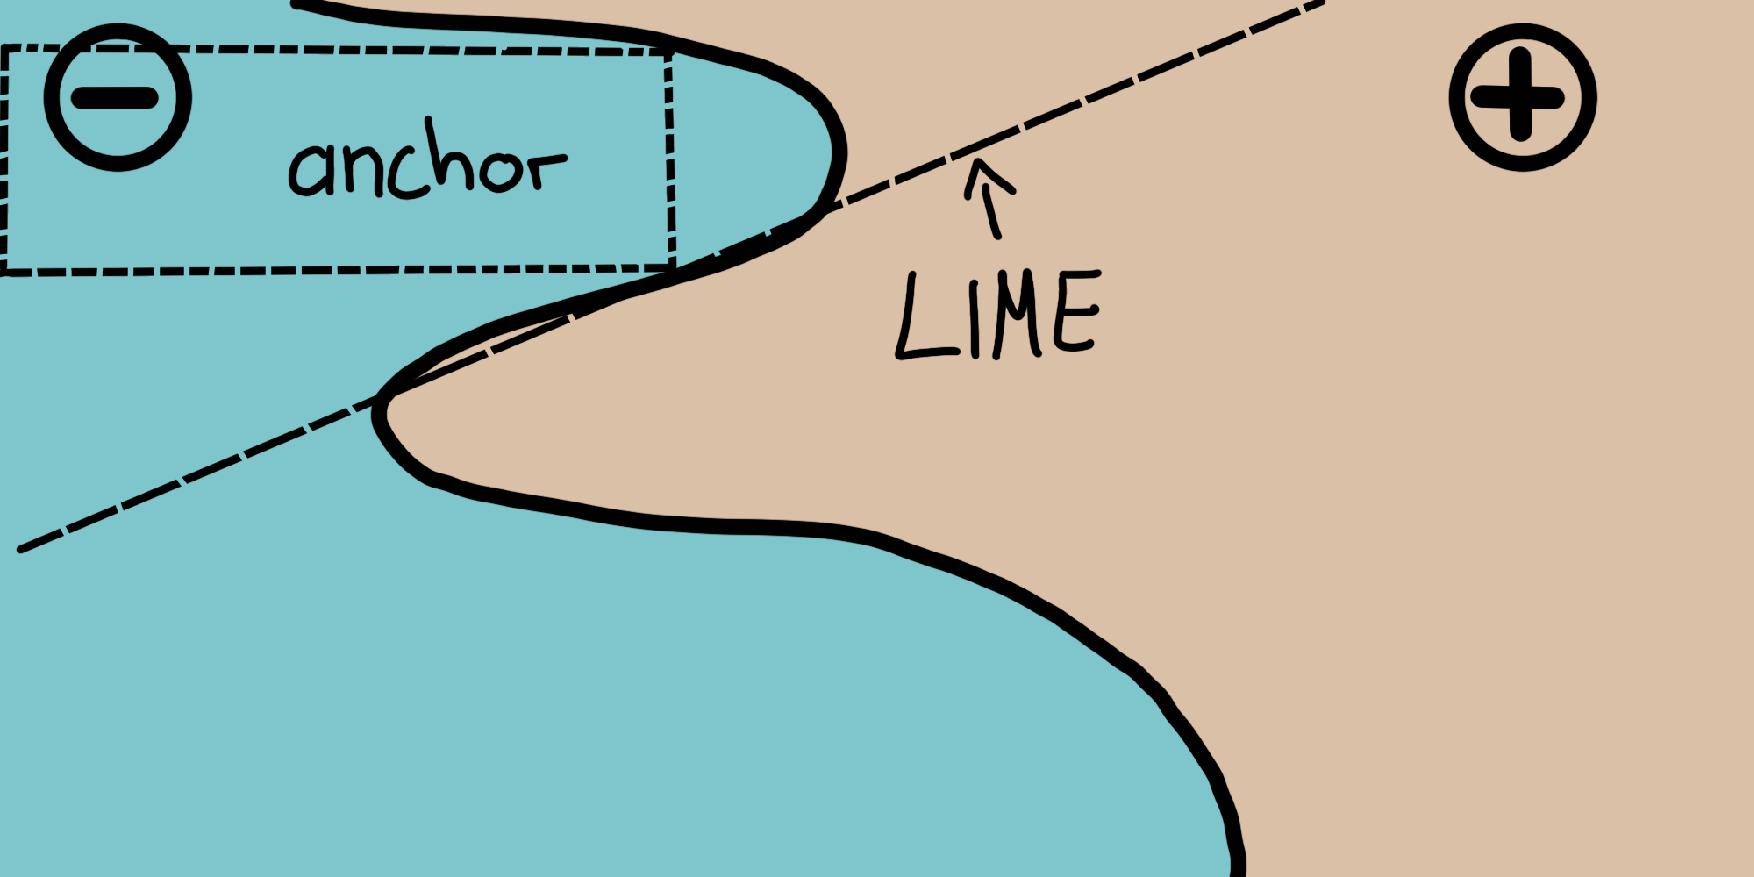
\includegraphics[width=200pt]{figures/figure_23.pdf}
\caption{A comparison between \ac{LIME} and anchors \cite{anchors}. One can see that, while \ac{LIME} tries its best to approximate the decision boundary's behaviour, an anchor provides a more realistic result.}
\label{fig:anchors_1}
\end{figure}

The form of an anchor is usually:\\

IF (feature$_{1}$ == value$_{1}$ AND/OR feature$_{2}$ == value$_{2}$ AND/OR ...) THEN \newline
PREDICT target = value$_{3}$ \newline
WITH PRECISION ...\% AND COVERAGE ...\%\\

The example above shows the readability provided by an anchor, which specifies the features that contributed the most to a prediction, the original model's prediction, the level of precision (i.e., accuracy) shown by the anchor and how applicable it is to the perturbation space's instances.

In more formal terms, an anchor $A$ must satisfy a given level of precision ($\tau$) such that $\text{precision}(A) \geqslant \tau$. To determine an anchor's precision, we can use the following equation:
\begin{equation}
    \text{precision}(A) = \mathbb{E}_{D(\mathbf{z}|A)}[\mathds{1}_{f(x)=f(\mathbf{z})}]
    \label{eq:13}
\end{equation}

Analysing equation \ref{eq:13}, $\mathbf{z}$ stands for the perturbed neighbours of $x$ to which $A$ is applicable, $D$ is the distribution of perturbed instances and $\mathds{1}_{f(x)=f(\mathbf{z})}$ denotes the black-box model's predictions with respect to $x$ and $\mathbf{z}$ (expectably, the same). In practice, it is intractable to determine adequate anchors using equation \ref{eq:13}. To solve such issue, the authors propose the introduction of a new parameter (referred to as $\delta$) such that $0 \leqslant \delta \leqslant 1$, effectively creating a probabilistic definition:
\begin{equation}
    P(\text{precision}(A) \geqslant \tau) \geqslant 1 - \delta
    \label{eq:14}
\end{equation}

Furthermore, the notion of coverage, intuitively explained as the need for rules that are applicable to a large portion of $D$, can also be described with an equation:
\begin{equation}
    \text{coverage}(A) = \E_{D_{(\mathbf{z})}}[A(\mathbf{z})]
    \label{eq:15}
\end{equation}

Maximising coverage is desirable, given that the generated anchors should be reusable on a decently sized portion of the perturbation space:
\begin{equation}
    \max_{\text{A s.t.} P(\text{precision}(A) \geqslant \tau) \geqslant 1 - \delta} \text{coverage}(A)
    \label{eq:16}
\end{equation}

From all the equations shown, it becomes clear that this process tries to find anchors with the highest coverage, assuming they satisfy the precision constraint (\ref{eq:14}). One interesting aspect is that, rules with more predicates (i.e., conditions in the IF branch) have a tendency for higher precision. However, such characteristic is not to be pushed to extreme cases. A rule that has too many predicates may be overly tuned to predict the instance given ($x$) and none other (or a really small amount of similar instances). There is, then, a trade-off between precision and coverage. \\

In addition to the formulations described above, this technique relies on the following steps:

\begin{enumerate}
    \item Candidate anchors are generated in rounds. The first round is responsible for creating one candidate per feature of $x$.
    \item The best performing candidates move to the next round, where they are expanded to explain yet another feature of $x$.
    \item This iterative process eventually stops when another routine determines we have an anchor good enough to satisfy equation \ref{eq:14}.
\end{enumerate} 

When an anchor is said to perform better than the remaining ones in any given round, a step was used involving the  Multi-Armed-Bandit formulation, where each arm is a candidate rule and a classical problem of exploration and exploitation arises. This type of setting helps speed up the search for an optimal rule, at any given moment.\\

In terms of examples, the original paper describes the process of obtaining anchors for text and image classification purposes (among other tasks), showing the versatility of this method. Text data is perturbed by omitting certain words and replacing them with pseudo-random ones (following some rules that guarantee coherent replacement words). As for images, instead of turning super-pixels on or off (as was the case with \ac{LIME}), the active ones are kept and superimposed over an unrelated image, to determine how the black-box model handles them:

\begin{figure}[h]
\centering
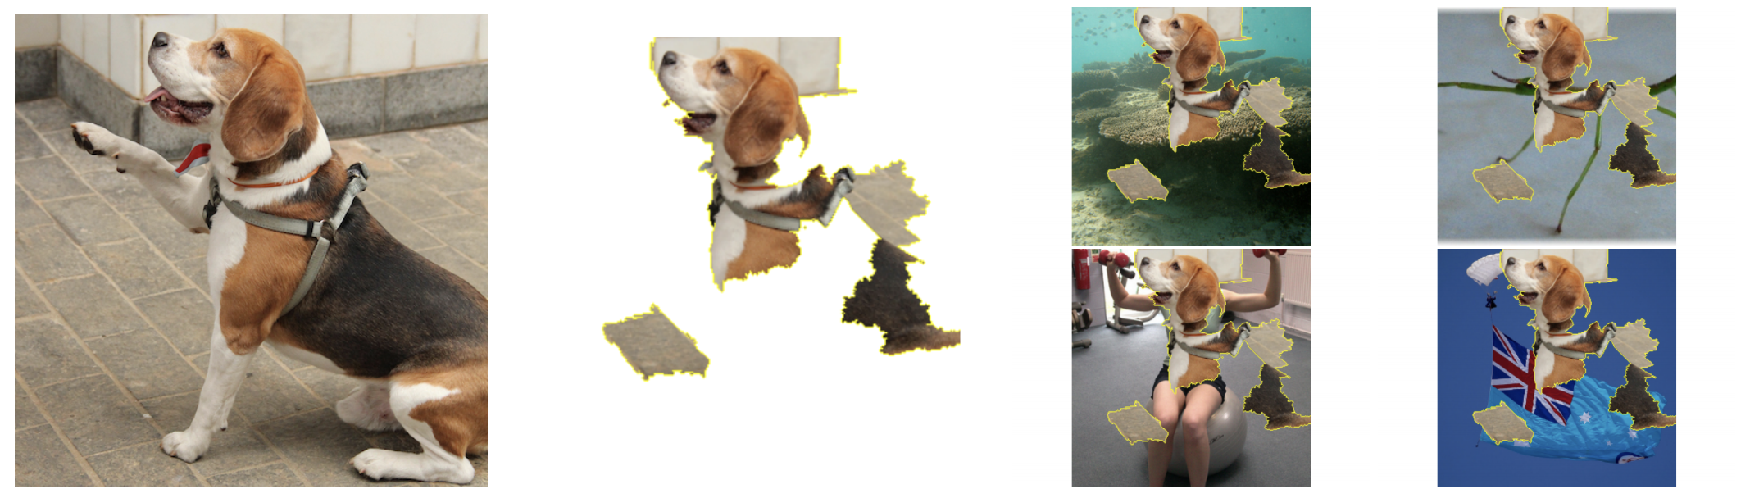
\includegraphics[width=390pt]{figures/figure_24.pdf}
\caption{Anchor explanations for the class "beagle" \cite{anchors}. In the rightmost figures, we can visualise how this technique superimposes the active super-pixels over unrelated samples to mislead a \ac{CNN}.}
\label{fig:anchors_2}
\end{figure}

Anchors are intuitive and easy to understand, delivering a performance level close to \ac{LIME}'s. Subsection \ref{subsec:chap4_explainability_evaluation} includes some experimental results with \ac{LIME}, instead of anchors, mainly due to the fact that there is an official implementation of \ac{LIME} for image data, but not for anchors.

\subsection{SHapley Additive exPlanations}
\label{subsec:chap2_shapley_additive_explanations}
\ac{SHAP}, first introduced in \cite{shap}, has its foundation laid upon Shapley values, which in turn originated from cooperative game theory. Here, features are seen as players inside a potentially collaborative environment, where they can choose to form coalitions (i.e., cooperative parties) to maximise future gains. 

As seen in the original source, to calculate the Shapley value for feature/player $i$, one can use the following formula:
\begin{equation}
    \boldsymbol{\phi}_{i} = \sum_{S \subseteq F \setminus \{i\}} \frac{|S|!(|F| - |S| - 1)!}{|F|!}[f_{S \cup \{i\}}(\mathbf{x}_{S \cup \{i\}}) - f_{S}(\mathbf{x}_{S})]
    \label{eq:17}
\end{equation}
Breaking down equation \ref{eq:17} step by step, we consider $F$ to be the set containing every feature in our problem and $S$ is some subset of $F$ that does not contain $i$. Additionally, $\mathbf{x}$ is the instance we seek to explain and $f$ is a version of the black-box model that considers $n$ features (for example, $f_{S \cup \{i\}}$ is a model that was trained to used all features in $S$ and $i$, but $f_{S}$ was trained exclusively with $S$). Hence, this method requires retraining $f$ for every possible coalition of the features present in $F$.\\

Starting from the right, with $[f_{S \cup \{i\}}(\mathbf{x}_{S \cup \{i\}}) - f_{S}(\mathbf{x}_{S})]$ we are computing the marginal value of adding player $i$ to subset $S$. In other words, we have a coalition where $i$ was not originally present ($S$), allowing us to perform a prediction using $f_{S}$ on $\mathbf{x}_{S}$. The obtained prediction is our base value (i.e., one where $i$ has no influence whatsoever). Then, if we train a version of the black-box model $f$ that uses $i$ ($f_{S \cup \{i\}}$) and give it an instance $\mathbf{x}_{S \cup \{i\}}$, we will get a prediction where feature $i$ was considered. Therefore, by subtracting this latter value by the former base value, we determine the marginal influence of feature $i$ in the game and feature subset $S$. 

Moving to the left, the fraction $\frac{|S|!(|F| - |S| - 1)!}{|F|!}$ is responsible for averaging out the effect of every other feature in $S$ that is not $i$. Imagining that $|S| = 3$ and $|F| = 5$, we would have $\frac{3!(5 - 3 - 1)!}{5!} = \frac{1}{20}$. Hence, every possible subset $S$ with three elements, derived from a set $F$ with five elements, contributes by $\frac{1}{20}$. This factor will then rescale the influence of $i$ in a specific subset $S$. By doing so, we are marginalising the actual composition of $S$, thus isolating the effect of feature $i$.

Finally, the summation repeats the same process for every possible subset $S$, essentially approximating the real Shapley value of feature $i$.\\

With the theoretical foundation provided above, one can understand \ac{SHAP} that much better. As the authors mention, \ac{SHAP} borrows from \ac{LIME} and Shapley values to build a better technique. Similarly to \ac{LIME}, \ac{SHAP} uses an auxiliary (linear) model to aid in the search for explanations. One interesting aspect of \ac{SHAP}, are the several branches that build upon it, like Kernel\ac{SHAP} \cite{molnar2019}, whose details will be described below.\\

Being based on a linear model that requires a training stage, the first step to understanding Kernel\ac{SHAP} is to analyse its loss function:
\begin{equation}
    L(f,g,\pi_{x}) = \sum_{\mathbf{z'} \in Z} [f(h_{x}(\mathbf{z'})) - g(\mathbf{z'})]^{2}\pi_{x}(\mathbf{z'})
    \label{eq:18}
\end{equation}
The main aspects of equation \ref{eq:18} are $f$ (the original black-box model), $g$ (the surrogate model) and $\pi_{x}$ (the \ac{SHAP} kernel).
The model $f$ can, basically, be any \ac{ML} model (i.e., we are only interested in what comes out of it). The same cannot be said about $g$, which is much more important for this technique and can be defined as:
\begin{equation}
    g(\mathbf{z}') = \boldsymbol{\phi}_{0} + \sum_{i = 1}^{m} \boldsymbol{\phi}_{i}\mathbf{z}'_{i}
    \label{eq:19}
\end{equation}
In the equation above, $g$ is, as we know, the explanation (surrogate) model, $\mathbf{z}'$ is a simplified vector of ones and zeros to enable or disable certain features (also known as the coalition vector), $M$ is the maximum coalition size and $\boldsymbol{\phi}_i$ is the coefficient (i.e., Shapley value) for feature $i$. For tabular data, the coalition vector would turn on or off certain features and for images it would do the same process but for super-pixels. According to \cite{shap}, formulation \ref{eq:19} has certain properties, amongst which, local accuracy (i.e., the explanation model should match the original model in terms of predictions).\\

The final piece of the puzzle is the \ac{SHAP} kernel, responsible for attributing more weight to small or large coalitions, as opposed to coalitions that only aggregate half the features (or close to it). We happen to learn more about individual features if we can analyse them in isolation (small coalitions) or if we have almost every feature but one (large  coalitions):
\begin{equation}
    \pi_{x}(\mathbf{z}') = \frac{(m - 1)}{\binom{m}{|\mathbf{z}'|}|\mathbf{z}'|(m - |\mathbf{z}'|)}
    \label{eq:20}
\end{equation}

Finally, the five steps that bring everything together are as follows:

\begin{enumerate}
    \item Sample $k$ coalitions: $\mathbf{z}'_{i} \in \{0,1\}^m, 0 \leq i < k$.
    \item Obtain predictions for each $\mathbf{z}'_{i}$ by using $f(h_x(\mathbf{z}'_{i}))$. Note that $h$ is a function that enables or disables features to form coalitions. For tabular data, it keeps the features we wish to form a coalition with and, for the deactivated features, it samples values from other instances. As for images, it keeps super-pixels (if they are paired with a $1$ in the coalition vector) or replaces them with a solid colour (if paired with a $0$).
    \item Compute the weight for each $\mathbf{z}'_{i}$ with equation \ref{eq:20}.
    \item Fit the weighted linear model using equation \ref{eq:18}.
    \item Return the coefficients from the linear model, namely, the Shapley values $\boldsymbol{\phi}$.
\end{enumerate}

After training, the computed coefficients ($\boldsymbol{\phi}$) are the Shapley values that explain each feature's effect over a sample's prediction. In order to illustrate the way Kernel\ac{SHAP} works, the following figure contains a visual explanation of a \ac{CNN}'s prediction:

\begin{figure}[h]
\centering
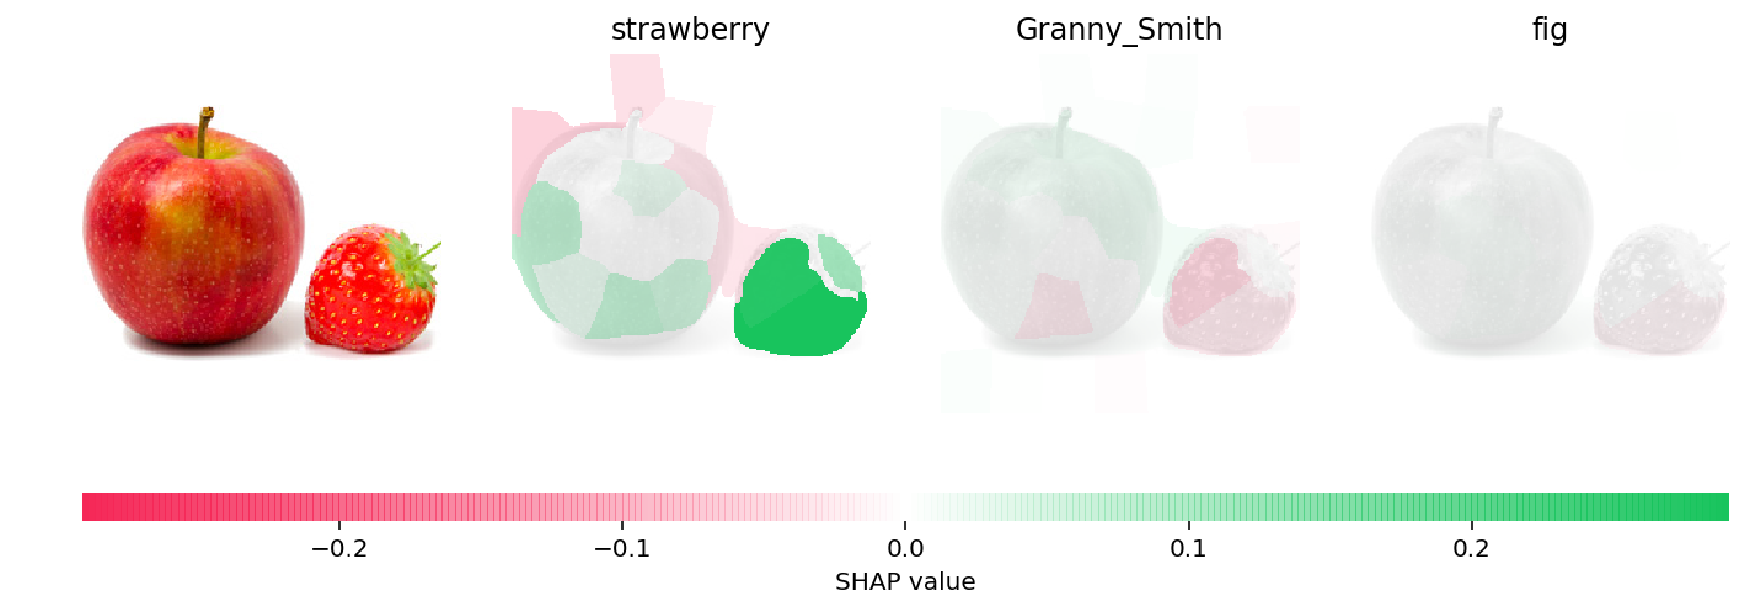
\includegraphics[width=380pt]{figures/figure_25.pdf}
\caption{Kernel\ac{SHAP}'s explanations of a \ac{CNN}'s predictions when given an image from the ImageNet dataset \cite{shap}. Green super-pixels have higher Shapley values and thus contribute more to the predicted class (unlike super-pixels marked with red tones - this behaviour is inverted in subsection \ref{subsec:chap4_explainability_evaluation}).}
\label{fig:shap}
\end{figure}

\ac{SHAP} is a solid technique with comparable results to \ac{LIME}'s, exceeding it in some cases. Additionally, it relies on grounded and proven concepts, like game theory, Shapley values and \ac{LIME}'s reasoning. However, Kernel\ac{SHAP} suffers much the same problems as other permutation based methods: by replacing omitted features with random ones, unlikely data points may be generated, which can lead to unrealistic explanations \cite{molnar2019}. \\

Nonetheless, a possible application of \ac{SHAP} to the problem of periocular recognition can be found in subsection \ref{subsec:chap4_explainability_evaluation}.

\section{Conclusion}
\label{sec:chap2_conclusion}

The present chapter focused on describing \ac{DL} and some of its main architectures, which lay the foundation for the proposed methods. Such description was followed by a compilation of the most relevant techniques in the field of \ac{ML} Explainability. Some of them are perfectly valid and interesting, but their applicability is let down by the lack of visual explanations or overly simple nature, while others are better suited to what this work is trying to accomplish. As an attempt to empirically validate this belief, the following chapter contemplates a section solely dedicated to discussing what results can be expected by only using existing techniques, in the search for an adequate level of explainability.